\documentclass[twoside]{book}

% Packages required by doxygen
\usepackage{calc}
\usepackage{doxygen}
\usepackage{graphicx}
\usepackage[utf8]{inputenc}
\usepackage{makeidx}
\usepackage{multicol}
\usepackage{multirow}
\usepackage{textcomp}
\usepackage[table]{xcolor}

% Font selection
\usepackage[T1]{fontenc}
\usepackage{mathptmx}
\usepackage[scaled=.90]{helvet}
\usepackage{courier}
\usepackage{amssymb}
\usepackage{sectsty}
\renewcommand{\familydefault}{\sfdefault}
\allsectionsfont{%
  \fontseries{bc}\selectfont%
  \color{darkgray}%
}
\renewcommand{\DoxyLabelFont}{%
  \fontseries{bc}\selectfont%
  \color{darkgray}%
}

% Page & text layout
\usepackage{geometry}
\geometry{%
  a4paper,%
  top=2.5cm,%
  bottom=2.5cm,%
  left=2.5cm,%
  right=2.5cm%
}
\tolerance=750
\hfuzz=15pt
\hbadness=750
\setlength{\emergencystretch}{15pt}
\setlength{\parindent}{0cm}
\setlength{\parskip}{0.2cm}
\makeatletter
\renewcommand{\paragraph}{%
  \@startsection{paragraph}{4}{0ex}{-1.0ex}{1.0ex}{%
    \normalfont\normalsize\bfseries\SS@parafont%
  }%
}
\renewcommand{\subparagraph}{%
  \@startsection{subparagraph}{5}{0ex}{-1.0ex}{1.0ex}{%
    \normalfont\normalsize\bfseries\SS@subparafont%
  }%
}
\makeatother

% Headers & footers
\usepackage{fancyhdr}
\pagestyle{fancyplain}
\fancyhead[LE]{\fancyplain{}{\bfseries\thepage}}
\fancyhead[CE]{\fancyplain{}{}}
\fancyhead[RE]{\fancyplain{}{\bfseries\leftmark}}
\fancyhead[LO]{\fancyplain{}{\bfseries\rightmark}}
\fancyhead[CO]{\fancyplain{}{}}
\fancyhead[RO]{\fancyplain{}{\bfseries\thepage}}
\fancyfoot[LE]{\fancyplain{}{}}
\fancyfoot[CE]{\fancyplain{}{}}
\fancyfoot[RE]{\fancyplain{}{\bfseries\scriptsize Generated on Mon Apr 4 2016 09\-:06\-:39 for My Project by Doxygen }}
\fancyfoot[LO]{\fancyplain{}{\bfseries\scriptsize Generated on Mon Apr 4 2016 09\-:06\-:39 for My Project by Doxygen }}
\fancyfoot[CO]{\fancyplain{}{}}
\fancyfoot[RO]{\fancyplain{}{}}
\renewcommand{\footrulewidth}{0.4pt}
\renewcommand{\chaptermark}[1]{%
  \markboth{#1}{}%
}
\renewcommand{\sectionmark}[1]{%
  \markright{\thesection\ #1}%
}

% Indices & bibliography
\usepackage{natbib}
\usepackage[titles]{tocloft}
\setcounter{tocdepth}{3}
\setcounter{secnumdepth}{5}
\makeindex

% Hyperlinks (required, but should be loaded last)
\usepackage{ifpdf}
\ifpdf
  \usepackage[pdftex,pagebackref=true]{hyperref}
\else
  \usepackage[ps2pdf,pagebackref=true]{hyperref}
\fi
\hypersetup{%
  colorlinks=true,%
  linkcolor=blue,%
  citecolor=blue,%
  unicode%
}

% Custom commands
\newcommand{\clearemptydoublepage}{%
  \newpage{\pagestyle{empty}\cleardoublepage}%
}


%===== C O N T E N T S =====

\begin{document}

% Titlepage & ToC
\hypersetup{pageanchor=false}
\pagenumbering{roman}
\begin{titlepage}
\vspace*{7cm}
\begin{center}%
{\Large My Project }\\
\vspace*{1cm}
{\large Generated by Doxygen 1.8.6}\\
\vspace*{0.5cm}
{\small Mon Apr 4 2016 09:06:39}\\
\end{center}
\end{titlepage}
\clearemptydoublepage
\tableofcontents
\clearemptydoublepage
\pagenumbering{arabic}
\hypersetup{pageanchor=true}

%--- Begin generated contents ---
\chapter{Namespace Index}
\section{Namespace List}
Here is a list of all documented namespaces with brief descriptions\-:\begin{DoxyCompactList}
\item\contentsline{section}{\hyperlink{namespaceed}{ed} }{\pageref{namespaceed}}{}
\end{DoxyCompactList}

\chapter{Hierarchical Index}
\section{Class Hierarchy}
This inheritance list is sorted roughly, but not completely, alphabetically\-:\begin{DoxyCompactList}
\item \contentsline{section}{ed\-:\-:Monomio\-Interfaz}{\pageref{classed_1_1MonomioInterfaz}}{}
\begin{DoxyCompactList}
\item \contentsline{section}{ed\-:\-:Monomio}{\pageref{classed_1_1Monomio}}{}
\end{DoxyCompactList}
\item \contentsline{section}{ed\-:\-:Polinomio\-Interfaz}{\pageref{classed_1_1PolinomioInterfaz}}{}
\begin{DoxyCompactList}
\item \contentsline{section}{ed\-:\-:Polinomio}{\pageref{classed_1_1Polinomio}}{}
\end{DoxyCompactList}
\end{DoxyCompactList}

\chapter{Class Index}
\section{Class List}
Here are the classes, structs, unions and interfaces with brief descriptions\-:\begin{DoxyCompactList}
\item\contentsline{section}{\hyperlink{classed_1_1Monomio}{ed\-::\-Monomio} \\*Definición de la clase \hyperlink{classed_1_1Monomio}{Monomio} }{\pageref{classed_1_1Monomio}}{}
\item\contentsline{section}{\hyperlink{classed_1_1MonomioInterfaz}{ed\-::\-Monomio\-Interfaz} \\*Definición de la clase \hyperlink{classed_1_1MonomioInterfaz}{Monomio\-Interfaz} }{\pageref{classed_1_1MonomioInterfaz}}{}
\item\contentsline{section}{\hyperlink{classed_1_1Polinomio}{ed\-::\-Polinomio} \\*Definición de la clase \hyperlink{classed_1_1Polinomio}{Polinomio} }{\pageref{classed_1_1Polinomio}}{}
\item\contentsline{section}{\hyperlink{classed_1_1PolinomioInterfaz}{ed\-::\-Polinomio\-Interfaz} \\*Definición de la clase \hyperlink{classed_1_1PolinomioInterfaz}{Polinomio\-Interfaz} }{\pageref{classed_1_1PolinomioInterfaz}}{}
\end{DoxyCompactList}

\chapter{File Index}
\section{File List}
Here is a list of all documented files with brief descriptions\-:\begin{DoxyCompactList}
\item\contentsline{section}{\hyperlink{macros_8hpp}{macros.\-hpp} \\*Macros para el diseño de pantallas }{\pageref{macros_8hpp}}{}
\item\contentsline{section}{{\bfseries monomio.\-hpp} }{\pageref{monomio_8hpp}}{}
\item\contentsline{section}{{\bfseries monomiointerfaz.\-hpp} }{\pageref{monomiointerfaz_8hpp}}{}
\item\contentsline{section}{{\bfseries polinomio.\-hpp} }{\pageref{polinomio_8hpp}}{}
\item\contentsline{section}{{\bfseries polinomio\-Interfaz.\-hpp} }{\pageref{polinomioInterfaz_8hpp}}{}
\end{DoxyCompactList}

\chapter{Namespace Documentation}
\hypertarget{namespaceed}{\section{ed Namespace Reference}
\label{namespaceed}\index{ed@{ed}}
}
\subsection*{Classes}
\begin{DoxyCompactItemize}
\item 
class \hyperlink{classed_1_1Monomio}{Monomio}
\begin{DoxyCompactList}\small\item\em Definición de la clase \hyperlink{classed_1_1Monomio}{Monomio}. \end{DoxyCompactList}\item 
class \hyperlink{classed_1_1MonomioInterfaz}{Monomio\-Interfaz}
\begin{DoxyCompactList}\small\item\em Definición de la clase \hyperlink{classed_1_1MonomioInterfaz}{Monomio\-Interfaz}. \end{DoxyCompactList}\item 
class \hyperlink{classed_1_1Polinomio}{Polinomio}
\begin{DoxyCompactList}\small\item\em Definición de la clase \hyperlink{classed_1_1Polinomio}{Polinomio}. \end{DoxyCompactList}\item 
class \hyperlink{classed_1_1PolinomioInterfaz}{Polinomio\-Interfaz}
\begin{DoxyCompactList}\small\item\em Definición de la clase \hyperlink{classed_1_1PolinomioInterfaz}{Polinomio\-Interfaz}. \end{DoxyCompactList}\end{DoxyCompactItemize}
\subsection*{Functions}
\begin{DoxyCompactItemize}
\item 
ostream \& \hyperlink{namespaceed_a741b43394bfe10620139a91ae65bf93c}{operator$<$$<$} (ostream \&stream, \hyperlink{classed_1_1Monomio}{Monomio} const \&p)
\item 
istream \& \hyperlink{namespaceed_afe8742ffe980d202ce5c6d3bc9a0aea3}{operator$>$$>$} (istream \&stream, \hyperlink{classed_1_1Monomio}{Monomio} \&p)
\item 
ostream \& \hyperlink{namespaceed_a7e9c987335ee267d8c9d405a9b36b87f}{operator$<$$<$} (ostream \&stream, \hyperlink{classed_1_1Polinomio}{Polinomio} const \&p)
\item 
istream \& \hyperlink{namespaceed_adf08b7a71eb5c75b9a1032e42cbf3215}{operator$>$$>$} (istream \&stream, \hyperlink{classed_1_1Polinomio}{Polinomio} \&p)
\end{DoxyCompactItemize}


\subsection{Detailed Description}
\begin{DoxyAttention}{Attention}
Se incluye la clase \hyperlink{classed_1_1Monomio}{Monomio} dentro del espacio de nombre ed

Se incluye la clase \hyperlink{classed_1_1Polinomio}{Polinomio} dentro del espacio de nombre ed 
\end{DoxyAttention}


\subsection{Function Documentation}
\hypertarget{namespaceed_a741b43394bfe10620139a91ae65bf93c}{\index{ed@{ed}!operator$<$$<$@{operator$<$$<$}}
\index{operator$<$$<$@{operator$<$$<$}!ed@{ed}}
\subsubsection[{operator$<$$<$}]{\setlength{\rightskip}{0pt plus 5cm}ostream\& ed\-::operator$<$$<$ (
\begin{DoxyParamCaption}
\item[{ostream \&}]{stream, }
\item[{{\bf Monomio} const \&}]{p}
\end{DoxyParamCaption}
)}}\label{namespaceed_a741b43394bfe10620139a91ae65bf93c}
\begin{DoxyAttention}{Attention}
Funcion amiga de la clase \hyperlink{classed_1_1Monomio}{Monomio} 
\end{DoxyAttention}

\begin{DoxyParams}{Parameters}
{\em stream} & ostream, flujo de salida \\
\hline
{\em p} & \hyperlink{classed_1_1Monomio}{Monomio}, pasado por referencia constante \\
\hline
\end{DoxyParams}
\begin{DoxyPrecond}{Precondition}
El monomio debe existir 
\end{DoxyPrecond}
\begin{DoxyPostcond}{Postcondition}
Se escribe por pantalla el coeficiente y el grado de un monomio 
\end{DoxyPostcond}
\begin{DoxySeeAlso}{See Also}
operator $>$$>$ 
\end{DoxySeeAlso}
\hypertarget{namespaceed_a7e9c987335ee267d8c9d405a9b36b87f}{\index{ed@{ed}!operator$<$$<$@{operator$<$$<$}}
\index{operator$<$$<$@{operator$<$$<$}!ed@{ed}}
\subsubsection[{operator$<$$<$}]{\setlength{\rightskip}{0pt plus 5cm}ostream\& ed\-::operator$<$$<$ (
\begin{DoxyParamCaption}
\item[{ostream \&}]{stream, }
\item[{{\bf Polinomio} const \&}]{p}
\end{DoxyParamCaption}
)}}\label{namespaceed_a7e9c987335ee267d8c9d405a9b36b87f}
\begin{DoxyAttention}{Attention}
Funcion amiga de la clase \hyperlink{classed_1_1Polinomio}{Polinomio} 
\end{DoxyAttention}

\begin{DoxyParams}{Parameters}
{\em stream} & ostream, flujo de salida \\
\hline
{\em p} & \hyperlink{classed_1_1Polinomio}{Polinomio}, pasado por referencia constante \\
\hline
\end{DoxyParams}
\begin{DoxyPrecond}{Precondition}
El \hyperlink{classed_1_1Polinomio}{Polinomio} debe existir 
\end{DoxyPrecond}
\begin{DoxyPostcond}{Postcondition}
Se escribe por pantalla el \hyperlink{classed_1_1Polinomio}{Polinomio} 
\end{DoxyPostcond}
\begin{DoxySeeAlso}{See Also}
operator $>$$>$ 
\end{DoxySeeAlso}
\hypertarget{namespaceed_afe8742ffe980d202ce5c6d3bc9a0aea3}{\index{ed@{ed}!operator$>$$>$@{operator$>$$>$}}
\index{operator$>$$>$@{operator$>$$>$}!ed@{ed}}
\subsubsection[{operator$>$$>$}]{\setlength{\rightskip}{0pt plus 5cm}istream\& ed\-::operator$>$$>$ (
\begin{DoxyParamCaption}
\item[{istream \&}]{stream, }
\item[{{\bf Monomio} \&}]{p}
\end{DoxyParamCaption}
)}}\label{namespaceed_afe8742ffe980d202ce5c6d3bc9a0aea3}
\begin{DoxyAttention}{Attention}
Funcion amiga de la clase \hyperlink{classed_1_1Monomio}{Monomio} 
\end{DoxyAttention}

\begin{DoxyParams}{Parameters}
{\em stream} & istream, flujo de entrada \\
\hline
{\em p} & \hyperlink{classed_1_1Monomio}{Monomio}, pasado por referencia \\
\hline
\end{DoxyParams}
\begin{DoxyPrecond}{Precondition}
El monomio debe existir 
\end{DoxyPrecond}
\begin{DoxyPostcond}{Postcondition}
Se le asignan los valores coeficiente y grado a un monomio 
\end{DoxyPostcond}
\begin{DoxySeeAlso}{See Also}
operator $<$$<$ 
\end{DoxySeeAlso}
\hypertarget{namespaceed_adf08b7a71eb5c75b9a1032e42cbf3215}{\index{ed@{ed}!operator$>$$>$@{operator$>$$>$}}
\index{operator$>$$>$@{operator$>$$>$}!ed@{ed}}
\subsubsection[{operator$>$$>$}]{\setlength{\rightskip}{0pt plus 5cm}istream\& ed\-::operator$>$$>$ (
\begin{DoxyParamCaption}
\item[{istream \&}]{stream, }
\item[{{\bf Polinomio} \&}]{p}
\end{DoxyParamCaption}
)}}\label{namespaceed_adf08b7a71eb5c75b9a1032e42cbf3215}
\begin{DoxyAttention}{Attention}
Funcion amiga de la clase \hyperlink{classed_1_1Polinomio}{Polinomio} 
\end{DoxyAttention}

\begin{DoxyParams}{Parameters}
{\em stream} & istream, flujo de entrada \\
\hline
{\em p} & \hyperlink{classed_1_1Polinomio}{Polinomio}, pasado por referencia \\
\hline
\end{DoxyParams}
\begin{DoxyPrecond}{Precondition}
El \hyperlink{classed_1_1Polinomio}{Polinomio} debe existir 
\end{DoxyPrecond}
\begin{DoxyPostcond}{Postcondition}
Se le asignan los valores al polinomio 
\end{DoxyPostcond}
\begin{DoxySeeAlso}{See Also}
operator $<$$<$ 
\end{DoxySeeAlso}

\chapter{Class Documentation}
\hypertarget{classed_1_1Monomio}{\section{ed\-:\-:Monomio Class Reference}
\label{classed_1_1Monomio}\index{ed\-::\-Monomio@{ed\-::\-Monomio}}
}


Definición de la clase \hyperlink{classed_1_1Monomio}{Monomio}.  




{\ttfamily \#include $<$monomio.\-hpp$>$}

Inheritance diagram for ed\-:\-:Monomio\-:\begin{figure}[H]
\begin{center}
\leavevmode
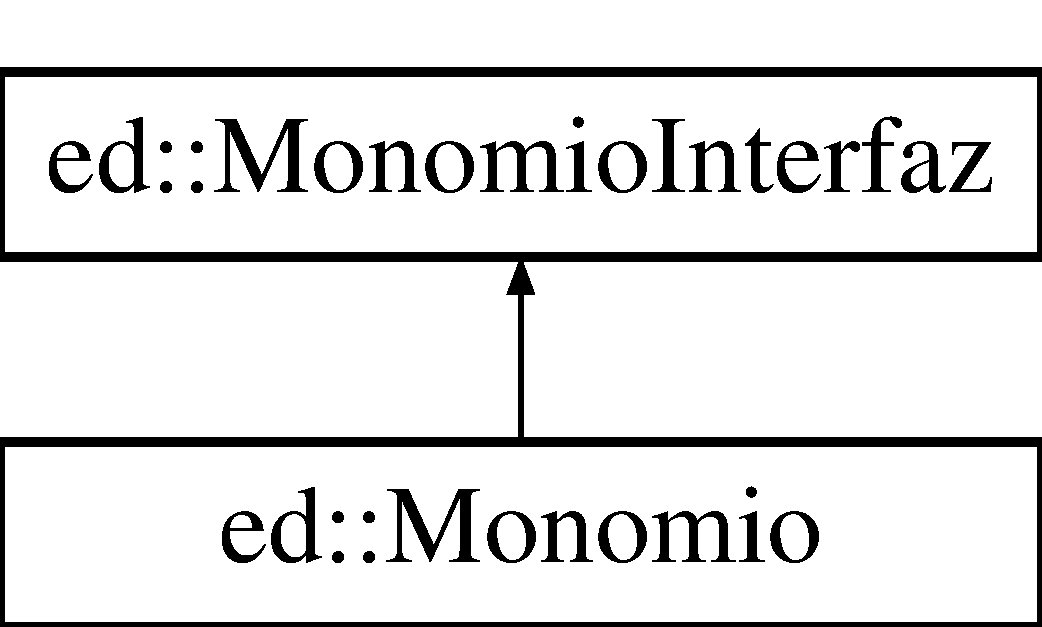
\includegraphics[height=2.000000cm]{classed_1_1Monomio}
\end{center}
\end{figure}
\subsection*{Public Member Functions}
\begin{Indent}{\bf Constructores de la clase Monomio}\par
\begin{DoxyCompactItemize}
\item 
\hyperlink{classed_1_1Monomio_ac11803dda1ae569b9ca4771187c9610a}{Monomio} (double coef=0.\-0, int grado=0)
\begin{DoxyCompactList}\small\item\em Contructor que crea un monomio a partir del coeficiente y del grado. \end{DoxyCompactList}\item 
\hyperlink{classed_1_1Monomio_a29ea5f824f31a241f2479ec40b60f0bd}{Monomio} (\hyperlink{classed_1_1Monomio}{Monomio} const \&p)
\begin{DoxyCompactList}\small\item\em Contructor que crea un monomio a partir de otro monomio pasado por referencia. \end{DoxyCompactList}\item 
double \hyperlink{classed_1_1Monomio_a1fa653597b00d3ebf69b26d84949051a}{get\-Coeficiente} () const 
\begin{DoxyCompactList}\small\item\em Devuelve el coeficiente de un monomio. \end{DoxyCompactList}\item 
int \hyperlink{classed_1_1Monomio_a22fd67c971fbbc239e882a0adc0f3ef2}{get\-Grado} () const 
\begin{DoxyCompactList}\small\item\em Devuelve el grado de un monomio. \end{DoxyCompactList}\item 
void \hyperlink{classed_1_1Monomio_a259fcdd7c96549aa053ffb4ac69af07f}{set\-Coeficiente} (const double \&coeficiente)
\begin{DoxyCompactList}\small\item\em Asigna un valor \char`\"{}coeficiente\char`\"{} al coeficiente de un monomio. \end{DoxyCompactList}\item 
void \hyperlink{classed_1_1Monomio_ae5ff9fdeb412ee9197f5395942d8ef47}{set\-Grado} (const int \&grado)
\begin{DoxyCompactList}\small\item\em Asigna un valor \char`\"{}grado\char`\"{} al grado de un monomio. \end{DoxyCompactList}\item 
\hyperlink{classed_1_1Monomio}{Monomio} \& \hyperlink{classed_1_1Monomio_a45103846ab828a1d4ff54cd723e14658}{operator=} (\hyperlink{classed_1_1Monomio}{Monomio} const \&p)
\begin{DoxyCompactList}\small\item\em /name Operadores \end{DoxyCompactList}\item 
\hyperlink{classed_1_1Monomio}{Monomio} \hyperlink{classed_1_1Monomio_a91a18ac215d83c32ab2803963441f79d}{operator$\ast$} (\hyperlink{classed_1_1Monomio}{Monomio} const \&p)
\begin{DoxyCompactList}\small\item\em Operador producto de dos monomios. \end{DoxyCompactList}\end{DoxyCompactItemize}
\end{Indent}
\begin{Indent}{\bf Funciones lectura y escritura de la clase Punto2\-D}\par
\begin{DoxyCompactItemize}
\item 
void \hyperlink{classed_1_1Monomio_a1d3ec4190c5e23d93eff79ad8e9486c0}{leer\-Monomio} ()
\begin{DoxyCompactList}\small\item\em Asigna el grado y el coeficiente a un monomio. \end{DoxyCompactList}\item 
void \hyperlink{classed_1_1Monomio_a42484a47d0d877232ee7775b97b1d480}{escribir\-Monomio} ()
\begin{DoxyCompactList}\small\item\em Escribe los valores de un monomio por pantalla. \end{DoxyCompactList}\item 
double \hyperlink{classed_1_1Monomio_a1fef28505a36f4ef961d47ab16281238}{valor\-Monomio} (double x)
\begin{DoxyCompactList}\small\item\em Calcula el valor de un monomio dado un valor x. \end{DoxyCompactList}\end{DoxyCompactItemize}
\end{Indent}
\subsection*{Friends}
\begin{Indent}{\bf Funciones amigas para poder acceder a la parte privada de Monomio}\par
\begin{DoxyCompactItemize}
\item 
ostream \& \hyperlink{classed_1_1Monomio_a35075baf54c0b258250d01e9ebc986b0}{operator$<$$<$} (ostream \&stream, \hyperlink{classed_1_1Monomio}{Monomio} const \&p)
\begin{DoxyCompactList}\small\item\em Sobrecarga del operador de salida \char`\"{}$<$$<$\char`\"{}. \end{DoxyCompactList}\item 
istream \& \hyperlink{classed_1_1Monomio_a1fcc0bb6adc11f90e3538f395c99c563}{operator$>$$>$} (istream \&stream, \hyperlink{classed_1_1Monomio}{Monomio} \&p)
\begin{DoxyCompactList}\small\item\em Sobrecarga del operador de entrada \char`\"{}$>$$>$\char`\"{}. \end{DoxyCompactList}\end{DoxyCompactItemize}
\end{Indent}


\subsection{Detailed Description}
Definición de la clase \hyperlink{classed_1_1Monomio}{Monomio}. 

\subsection{Constructor \& Destructor Documentation}
\hypertarget{classed_1_1Monomio_ac11803dda1ae569b9ca4771187c9610a}{\index{ed\-::\-Monomio@{ed\-::\-Monomio}!Monomio@{Monomio}}
\index{Monomio@{Monomio}!ed::Monomio@{ed\-::\-Monomio}}
\subsubsection[{Monomio}]{\setlength{\rightskip}{0pt plus 5cm}ed\-::\-Monomio\-::\-Monomio (
\begin{DoxyParamCaption}
\item[{double}]{coef = {\ttfamily 0.0}, }
\item[{int}]{grado = {\ttfamily 0}}
\end{DoxyParamCaption}
)\hspace{0.3cm}{\ttfamily [inline]}}}\label{classed_1_1Monomio_ac11803dda1ae569b9ca4771187c9610a}


Contructor que crea un monomio a partir del coeficiente y del grado. 

\begin{DoxyAttention}{Attention}
Función sobrecargada 
\end{DoxyAttention}
\begin{DoxyNote}{Note}
Los parámetros tienen valores por defecto 
\end{DoxyNote}

\begin{DoxyParams}{Parameters}
{\em coef} & double, valor por defecto 0.\-0 \\
\hline
{\em grado} & int, valor por defecto 0 \\
\hline
\end{DoxyParams}
\begin{DoxyPrecond}{Precondition}
Ninguna 
\end{DoxyPrecond}
\begin{DoxyPostcond}{Postcondition}
Ninguna 
\end{DoxyPostcond}
\begin{DoxySeeAlso}{See Also}
\hyperlink{classed_1_1Monomio_a259fcdd7c96549aa053ffb4ac69af07f}{set\-Coeficiente()}, \hyperlink{classed_1_1Monomio_ae5ff9fdeb412ee9197f5395942d8ef47}{set\-Grado()} 
\end{DoxySeeAlso}
\hypertarget{classed_1_1Monomio_a29ea5f824f31a241f2479ec40b60f0bd}{\index{ed\-::\-Monomio@{ed\-::\-Monomio}!Monomio@{Monomio}}
\index{Monomio@{Monomio}!ed::Monomio@{ed\-::\-Monomio}}
\subsubsection[{Monomio}]{\setlength{\rightskip}{0pt plus 5cm}ed\-::\-Monomio\-::\-Monomio (
\begin{DoxyParamCaption}
\item[{{\bf Monomio} const \&}]{p}
\end{DoxyParamCaption}
)\hspace{0.3cm}{\ttfamily [inline]}}}\label{classed_1_1Monomio_a29ea5f824f31a241f2479ec40b60f0bd}


Contructor que crea un monomio a partir de otro monomio pasado por referencia. 

\begin{DoxyAttention}{Attention}
Función sobrecargada 
\end{DoxyAttention}

\begin{DoxyParams}{Parameters}
{\em p} & \hyperlink{classed_1_1Monomio}{Monomio}, \hyperlink{classed_1_1Monomio}{Monomio} pasado por referencia \\
\hline
\end{DoxyParams}
\begin{DoxyPrecond}{Precondition}
Ninguna 
\end{DoxyPrecond}
\begin{DoxyPostcond}{Postcondition}
Ninguna 
\end{DoxyPostcond}
\begin{DoxySeeAlso}{See Also}
\hyperlink{classed_1_1Monomio_a259fcdd7c96549aa053ffb4ac69af07f}{set\-Coeficiente()}, \hyperlink{classed_1_1Monomio_ae5ff9fdeb412ee9197f5395942d8ef47}{set\-Grado()}, \hyperlink{classed_1_1Monomio_a22fd67c971fbbc239e882a0adc0f3ef2}{get\-Grado()}, \hyperlink{classed_1_1Monomio_a1fa653597b00d3ebf69b26d84949051a}{get\-Coeficiente()} 
\end{DoxySeeAlso}


\subsection{Member Function Documentation}
\hypertarget{classed_1_1Monomio_a42484a47d0d877232ee7775b97b1d480}{\index{ed\-::\-Monomio@{ed\-::\-Monomio}!escribir\-Monomio@{escribir\-Monomio}}
\index{escribir\-Monomio@{escribir\-Monomio}!ed::Monomio@{ed\-::\-Monomio}}
\subsubsection[{escribir\-Monomio}]{\setlength{\rightskip}{0pt plus 5cm}void Monomio\-::escribir\-Monomio (
\begin{DoxyParamCaption}
{}
\end{DoxyParamCaption}
)}}\label{classed_1_1Monomio_a42484a47d0d877232ee7775b97b1d480}


Escribe los valores de un monomio por pantalla. 

\begin{DoxyPrecond}{Precondition}
El monomio debe existir 
\end{DoxyPrecond}
\begin{DoxyPostcond}{Postcondition}
Ninguna 
\end{DoxyPostcond}
\begin{DoxySeeAlso}{See Also}
\hyperlink{classed_1_1Monomio_a22fd67c971fbbc239e882a0adc0f3ef2}{get\-Grado()}, \hyperlink{classed_1_1Monomio_a1fa653597b00d3ebf69b26d84949051a}{get\-Coeficiente()} 
\end{DoxySeeAlso}
\hypertarget{classed_1_1Monomio_a1fa653597b00d3ebf69b26d84949051a}{\index{ed\-::\-Monomio@{ed\-::\-Monomio}!get\-Coeficiente@{get\-Coeficiente}}
\index{get\-Coeficiente@{get\-Coeficiente}!ed::Monomio@{ed\-::\-Monomio}}
\subsubsection[{get\-Coeficiente}]{\setlength{\rightskip}{0pt plus 5cm}double ed\-::\-Monomio\-::get\-Coeficiente (
\begin{DoxyParamCaption}
{}
\end{DoxyParamCaption}
) const\hspace{0.3cm}{\ttfamily [inline]}, {\ttfamily [virtual]}}}\label{classed_1_1Monomio_a1fa653597b00d3ebf69b26d84949051a}


Devuelve el coeficiente de un monomio. 

\begin{DoxyReturn}{Returns}
Coeficiente de un monomio 
\end{DoxyReturn}
\begin{DoxyPrecond}{Precondition}
El monomio debe existir anteriormente 
\end{DoxyPrecond}
\begin{DoxyPostcond}{Postcondition}
Ninguna 
\end{DoxyPostcond}
\begin{DoxySeeAlso}{See Also}
\hyperlink{classed_1_1Monomio_a22fd67c971fbbc239e882a0adc0f3ef2}{get\-Grado()} 
\end{DoxySeeAlso}


Implements \hyperlink{classed_1_1MonomioInterfaz_a8dade5810b660860408169bca4b35e2e}{ed\-::\-Monomio\-Interfaz}.

\hypertarget{classed_1_1Monomio_a22fd67c971fbbc239e882a0adc0f3ef2}{\index{ed\-::\-Monomio@{ed\-::\-Monomio}!get\-Grado@{get\-Grado}}
\index{get\-Grado@{get\-Grado}!ed::Monomio@{ed\-::\-Monomio}}
\subsubsection[{get\-Grado}]{\setlength{\rightskip}{0pt plus 5cm}int ed\-::\-Monomio\-::get\-Grado (
\begin{DoxyParamCaption}
{}
\end{DoxyParamCaption}
) const\hspace{0.3cm}{\ttfamily [inline]}, {\ttfamily [virtual]}}}\label{classed_1_1Monomio_a22fd67c971fbbc239e882a0adc0f3ef2}


Devuelve el grado de un monomio. 

\begin{DoxyReturn}{Returns}
Grado de un monomio 
\end{DoxyReturn}
\begin{DoxyPrecond}{Precondition}
El monomio debe existir 
\end{DoxyPrecond}
\begin{DoxyPostcond}{Postcondition}
Ninguna 
\end{DoxyPostcond}
\begin{DoxySeeAlso}{See Also}
\hyperlink{classed_1_1Monomio_a1fa653597b00d3ebf69b26d84949051a}{get\-Coeficiente()} 
\end{DoxySeeAlso}


Implements \hyperlink{classed_1_1MonomioInterfaz_aa5b87185650a82784b39b9bbbaec7dcb}{ed\-::\-Monomio\-Interfaz}.

\hypertarget{classed_1_1Monomio_a1d3ec4190c5e23d93eff79ad8e9486c0}{\index{ed\-::\-Monomio@{ed\-::\-Monomio}!leer\-Monomio@{leer\-Monomio}}
\index{leer\-Monomio@{leer\-Monomio}!ed::Monomio@{ed\-::\-Monomio}}
\subsubsection[{leer\-Monomio}]{\setlength{\rightskip}{0pt plus 5cm}void Monomio\-::leer\-Monomio (
\begin{DoxyParamCaption}
{}
\end{DoxyParamCaption}
)}}\label{classed_1_1Monomio_a1d3ec4190c5e23d93eff79ad8e9486c0}


Asigna el grado y el coeficiente a un monomio. 

\begin{DoxyPrecond}{Precondition}
El monomio debe existir 
\end{DoxyPrecond}
\begin{DoxyPostcond}{Postcondition}
Ninguna 
\end{DoxyPostcond}
\begin{DoxySeeAlso}{See Also}
\hyperlink{classed_1_1Monomio_ae5ff9fdeb412ee9197f5395942d8ef47}{set\-Grado()}, \hyperlink{classed_1_1Monomio_a259fcdd7c96549aa053ffb4ac69af07f}{set\-Coeficiente()} 
\end{DoxySeeAlso}
\hypertarget{classed_1_1Monomio_a91a18ac215d83c32ab2803963441f79d}{\index{ed\-::\-Monomio@{ed\-::\-Monomio}!operator$\ast$@{operator$\ast$}}
\index{operator$\ast$@{operator$\ast$}!ed::Monomio@{ed\-::\-Monomio}}
\subsubsection[{operator$\ast$}]{\setlength{\rightskip}{0pt plus 5cm}{\bf Monomio} ed\-::\-Monomio\-::operator$\ast$ (
\begin{DoxyParamCaption}
\item[{{\bf Monomio} const \&}]{p}
\end{DoxyParamCaption}
)\hspace{0.3cm}{\ttfamily [inline]}}}\label{classed_1_1Monomio_a91a18ac215d83c32ab2803963441f79d}


Operador producto de dos monomios. 

\begin{DoxyAttention}{Attention}
Se sobrecarga el operador producto 
\end{DoxyAttention}

\begin{DoxyParams}{Parameters}
{\em p} & \hyperlink{classed_1_1Monomio}{Monomio} pasado por referencia constante \\
\hline
\end{DoxyParams}
\begin{DoxyPrecond}{Precondition}
El monomio debe existir 
\end{DoxyPrecond}
\begin{DoxyPostcond}{Postcondition}
Ninguna 
\end{DoxyPostcond}
\begin{DoxySeeAlso}{See Also}
\hyperlink{classed_1_1Monomio_a22fd67c971fbbc239e882a0adc0f3ef2}{get\-Grado()}, \hyperlink{classed_1_1Monomio_a1fa653597b00d3ebf69b26d84949051a}{get\-Coeficiente()}, \hyperlink{classed_1_1Monomio_ae5ff9fdeb412ee9197f5395942d8ef47}{set\-Grado()}, \hyperlink{classed_1_1Monomio_a259fcdd7c96549aa053ffb4ac69af07f}{set\-Coeficiente()} 
\end{DoxySeeAlso}
\hypertarget{classed_1_1Monomio_a45103846ab828a1d4ff54cd723e14658}{\index{ed\-::\-Monomio@{ed\-::\-Monomio}!operator=@{operator=}}
\index{operator=@{operator=}!ed::Monomio@{ed\-::\-Monomio}}
\subsubsection[{operator=}]{\setlength{\rightskip}{0pt plus 5cm}{\bf Monomio}\& ed\-::\-Monomio\-::operator= (
\begin{DoxyParamCaption}
\item[{{\bf Monomio} const \&}]{p}
\end{DoxyParamCaption}
)\hspace{0.3cm}{\ttfamily [inline]}}}\label{classed_1_1Monomio_a45103846ab828a1d4ff54cd723e14658}


/name Operadores 

Operador de copia de monomio en otro \begin{DoxyAttention}{Attention}
Se sobrecarga el operador de asignacion 
\end{DoxyAttention}

\begin{DoxyParams}{Parameters}
{\em p} & \hyperlink{classed_1_1Monomio}{Monomio} pasado por referencia constante \\
\hline
\end{DoxyParams}
\begin{DoxyPrecond}{Precondition}
El monomio debe existir 
\end{DoxyPrecond}
\begin{DoxyPostcond}{Postcondition}
Ninguna 
\end{DoxyPostcond}
\begin{DoxySeeAlso}{See Also}
\hyperlink{classed_1_1Monomio_a22fd67c971fbbc239e882a0adc0f3ef2}{get\-Grado()}, \hyperlink{classed_1_1Monomio_a1fa653597b00d3ebf69b26d84949051a}{get\-Coeficiente()}, \hyperlink{classed_1_1Monomio_ae5ff9fdeb412ee9197f5395942d8ef47}{set\-Grado()}, \hyperlink{classed_1_1Monomio_a259fcdd7c96549aa053ffb4ac69af07f}{set\-Coeficiente()} 
\end{DoxySeeAlso}
\hypertarget{classed_1_1Monomio_a259fcdd7c96549aa053ffb4ac69af07f}{\index{ed\-::\-Monomio@{ed\-::\-Monomio}!set\-Coeficiente@{set\-Coeficiente}}
\index{set\-Coeficiente@{set\-Coeficiente}!ed::Monomio@{ed\-::\-Monomio}}
\subsubsection[{set\-Coeficiente}]{\setlength{\rightskip}{0pt plus 5cm}void ed\-::\-Monomio\-::set\-Coeficiente (
\begin{DoxyParamCaption}
\item[{const double \&}]{coeficiente}
\end{DoxyParamCaption}
)\hspace{0.3cm}{\ttfamily [inline]}, {\ttfamily [virtual]}}}\label{classed_1_1Monomio_a259fcdd7c96549aa053ffb4ac69af07f}


Asigna un valor \char`\"{}coeficiente\char`\"{} al coeficiente de un monomio. 


\begin{DoxyParams}{Parameters}
{\em coeficiente} & double pasado por referencia constante \\
\hline
\end{DoxyParams}
\begin{DoxyPrecond}{Precondition}
El monomio debe existir 
\end{DoxyPrecond}
\begin{DoxyPostcond}{Postcondition}
Ninguna 
\end{DoxyPostcond}
\begin{DoxySeeAlso}{See Also}
\hyperlink{classed_1_1Monomio_ae5ff9fdeb412ee9197f5395942d8ef47}{set\-Grado()} 
\end{DoxySeeAlso}


Implements \hyperlink{classed_1_1MonomioInterfaz_a40ba6a0dc0940f60842a319f982aac6d}{ed\-::\-Monomio\-Interfaz}.

\hypertarget{classed_1_1Monomio_ae5ff9fdeb412ee9197f5395942d8ef47}{\index{ed\-::\-Monomio@{ed\-::\-Monomio}!set\-Grado@{set\-Grado}}
\index{set\-Grado@{set\-Grado}!ed::Monomio@{ed\-::\-Monomio}}
\subsubsection[{set\-Grado}]{\setlength{\rightskip}{0pt plus 5cm}void ed\-::\-Monomio\-::set\-Grado (
\begin{DoxyParamCaption}
\item[{const int \&}]{grado}
\end{DoxyParamCaption}
)\hspace{0.3cm}{\ttfamily [inline]}, {\ttfamily [virtual]}}}\label{classed_1_1Monomio_ae5ff9fdeb412ee9197f5395942d8ef47}


Asigna un valor \char`\"{}grado\char`\"{} al grado de un monomio. 


\begin{DoxyParams}{Parameters}
{\em grado} & int pasado por referencia constante \\
\hline
\end{DoxyParams}
\begin{DoxyPrecond}{Precondition}
El monomio debe existir 
\end{DoxyPrecond}
\begin{DoxyPostcond}{Postcondition}
Ninguna 
\end{DoxyPostcond}
\begin{DoxySeeAlso}{See Also}
\hyperlink{classed_1_1Monomio_a259fcdd7c96549aa053ffb4ac69af07f}{set\-Coeficiente()} 
\end{DoxySeeAlso}


Implements \hyperlink{classed_1_1MonomioInterfaz_a7294c2a6a1c76ef374202e45f54f1da6}{ed\-::\-Monomio\-Interfaz}.

\hypertarget{classed_1_1Monomio_a1fef28505a36f4ef961d47ab16281238}{\index{ed\-::\-Monomio@{ed\-::\-Monomio}!valor\-Monomio@{valor\-Monomio}}
\index{valor\-Monomio@{valor\-Monomio}!ed::Monomio@{ed\-::\-Monomio}}
\subsubsection[{valor\-Monomio}]{\setlength{\rightskip}{0pt plus 5cm}double Monomio\-::valor\-Monomio (
\begin{DoxyParamCaption}
\item[{double}]{x}
\end{DoxyParamCaption}
)}}\label{classed_1_1Monomio_a1fef28505a36f4ef961d47ab16281238}


Calcula el valor de un monomio dado un valor x. 


\begin{DoxyParams}{Parameters}
{\em x} & double \\
\hline
\end{DoxyParams}
\begin{DoxyPrecond}{Precondition}
El monomio debe existir 
\end{DoxyPrecond}
\begin{DoxyPostcond}{Postcondition}
Ninguna 
\end{DoxyPostcond}
\begin{DoxySeeAlso}{See Also}
\hyperlink{classed_1_1Monomio_a22fd67c971fbbc239e882a0adc0f3ef2}{get\-Grado()}, \hyperlink{classed_1_1Monomio_a1fa653597b00d3ebf69b26d84949051a}{get\-Coeficiente()} 
\end{DoxySeeAlso}


\subsection{Friends And Related Function Documentation}
\hypertarget{classed_1_1Monomio_a35075baf54c0b258250d01e9ebc986b0}{\index{ed\-::\-Monomio@{ed\-::\-Monomio}!operator$<$$<$@{operator$<$$<$}}
\index{operator$<$$<$@{operator$<$$<$}!ed::Monomio@{ed\-::\-Monomio}}
\subsubsection[{operator$<$$<$}]{\setlength{\rightskip}{0pt plus 5cm}ostream\& operator$<$$<$ (
\begin{DoxyParamCaption}
\item[{ostream \&}]{stream, }
\item[{{\bf Monomio} const \&}]{p}
\end{DoxyParamCaption}
)\hspace{0.3cm}{\ttfamily [friend]}}}\label{classed_1_1Monomio_a35075baf54c0b258250d01e9ebc986b0}


Sobrecarga del operador de salida \char`\"{}$<$$<$\char`\"{}. 

\begin{DoxyAttention}{Attention}
Funcion amiga de la clase \hyperlink{classed_1_1Monomio}{Monomio} 
\end{DoxyAttention}

\begin{DoxyParams}{Parameters}
{\em stream} & ostream, flujo de salida \\
\hline
{\em p} & \hyperlink{classed_1_1Monomio}{Monomio}, pasado por referencia constante \\
\hline
\end{DoxyParams}
\begin{DoxyPrecond}{Precondition}
El monomio debe existir 
\end{DoxyPrecond}
\begin{DoxyPostcond}{Postcondition}
Se escribe por pantalla el coeficiente y el grado de un monomio 
\end{DoxyPostcond}
\begin{DoxySeeAlso}{See Also}
operator $>$$>$ 
\end{DoxySeeAlso}
\hypertarget{classed_1_1Monomio_a1fcc0bb6adc11f90e3538f395c99c563}{\index{ed\-::\-Monomio@{ed\-::\-Monomio}!operator$>$$>$@{operator$>$$>$}}
\index{operator$>$$>$@{operator$>$$>$}!ed::Monomio@{ed\-::\-Monomio}}
\subsubsection[{operator$>$$>$}]{\setlength{\rightskip}{0pt plus 5cm}istream\& operator$>$$>$ (
\begin{DoxyParamCaption}
\item[{istream \&}]{stream, }
\item[{{\bf Monomio} \&}]{p}
\end{DoxyParamCaption}
)\hspace{0.3cm}{\ttfamily [friend]}}}\label{classed_1_1Monomio_a1fcc0bb6adc11f90e3538f395c99c563}


Sobrecarga del operador de entrada \char`\"{}$>$$>$\char`\"{}. 

\begin{DoxyAttention}{Attention}
Funcion amiga de la clase \hyperlink{classed_1_1Monomio}{Monomio} 
\end{DoxyAttention}

\begin{DoxyParams}{Parameters}
{\em stream} & istream, flujo de entrada \\
\hline
{\em p} & \hyperlink{classed_1_1Monomio}{Monomio}, pasado por referencia \\
\hline
\end{DoxyParams}
\begin{DoxyPrecond}{Precondition}
El monomio debe existir 
\end{DoxyPrecond}
\begin{DoxyPostcond}{Postcondition}
Se le asignan los valores coeficiente y grado a un monomio 
\end{DoxyPostcond}
\begin{DoxySeeAlso}{See Also}
operator $<$$<$ 
\end{DoxySeeAlso}


The documentation for this class was generated from the following files\-:\begin{DoxyCompactItemize}
\item 
monomio.\-hpp\item 
monomio.\-cpp\end{DoxyCompactItemize}

\hypertarget{classed_1_1MonomioInterfaz}{\section{ed\-:\-:Monomio\-Interfaz Class Reference}
\label{classed_1_1MonomioInterfaz}\index{ed\-::\-Monomio\-Interfaz@{ed\-::\-Monomio\-Interfaz}}
}


Definición de la clase \hyperlink{classed_1_1MonomioInterfaz}{Monomio\-Interfaz}.  




{\ttfamily \#include $<$monomiointerfaz.\-hpp$>$}

Inheritance diagram for ed\-:\-:Monomio\-Interfaz\-:\begin{figure}[H]
\begin{center}
\leavevmode
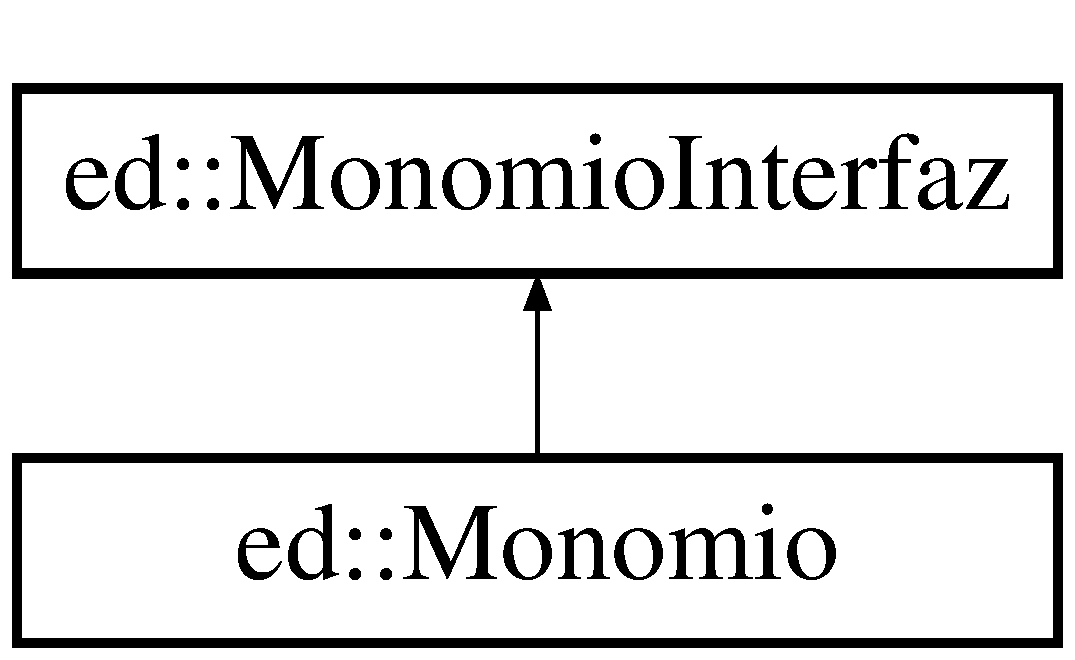
\includegraphics[height=2.000000cm]{classed_1_1MonomioInterfaz}
\end{center}
\end{figure}
\subsection*{Public Member Functions}
\begin{Indent}{\bf Métodos públicos de la clase Monomio}\par
\begin{DoxyCompactItemize}
\item 
virtual double \hyperlink{classed_1_1MonomioInterfaz_a8dade5810b660860408169bca4b35e2e}{get\-Coeficiente} () const =0
\begin{DoxyCompactList}\small\item\em Devuelve el coeficiente de un monomio. \end{DoxyCompactList}\item 
virtual int \hyperlink{classed_1_1MonomioInterfaz_aa5b87185650a82784b39b9bbbaec7dcb}{get\-Grado} () const =0
\begin{DoxyCompactList}\small\item\em Devuelve el grado de un monomio. \end{DoxyCompactList}\item 
virtual void \hyperlink{classed_1_1MonomioInterfaz_a40ba6a0dc0940f60842a319f982aac6d}{set\-Coeficiente} (const double \&coeficiente)=0
\begin{DoxyCompactList}\small\item\em Asigna un valor \char`\"{}coeficiente\char`\"{} al coeficiente de un monomio. \end{DoxyCompactList}\item 
virtual void \hyperlink{classed_1_1MonomioInterfaz_a7294c2a6a1c76ef374202e45f54f1da6}{set\-Grado} (const int \&grado)=0
\begin{DoxyCompactList}\small\item\em Asigna un valor \char`\"{}grado\char`\"{} al grado de un monomio. \end{DoxyCompactList}\end{DoxyCompactItemize}
\end{Indent}


\subsection{Detailed Description}
Definición de la clase \hyperlink{classed_1_1MonomioInterfaz}{Monomio\-Interfaz}. 

\subsection{Member Function Documentation}
\hypertarget{classed_1_1MonomioInterfaz_a8dade5810b660860408169bca4b35e2e}{\index{ed\-::\-Monomio\-Interfaz@{ed\-::\-Monomio\-Interfaz}!get\-Coeficiente@{get\-Coeficiente}}
\index{get\-Coeficiente@{get\-Coeficiente}!ed::MonomioInterfaz@{ed\-::\-Monomio\-Interfaz}}
\subsubsection[{get\-Coeficiente}]{\setlength{\rightskip}{0pt plus 5cm}virtual double ed\-::\-Monomio\-Interfaz\-::get\-Coeficiente (
\begin{DoxyParamCaption}
{}
\end{DoxyParamCaption}
) const\hspace{0.3cm}{\ttfamily [pure virtual]}}}\label{classed_1_1MonomioInterfaz_a8dade5810b660860408169bca4b35e2e}


Devuelve el coeficiente de un monomio. 

\begin{DoxyReturn}{Returns}
Coeficiente de un monomio 
\end{DoxyReturn}
\begin{DoxyPrecond}{Precondition}
El monomio debe existir anteriormente 
\end{DoxyPrecond}
\begin{DoxyPostcond}{Postcondition}
Ninguna 
\end{DoxyPostcond}
\begin{DoxySeeAlso}{See Also}
\hyperlink{classed_1_1MonomioInterfaz_aa5b87185650a82784b39b9bbbaec7dcb}{get\-Grado()} 
\end{DoxySeeAlso}


Implemented in \hyperlink{classed_1_1Monomio_a1fa653597b00d3ebf69b26d84949051a}{ed\-::\-Monomio}.

\hypertarget{classed_1_1MonomioInterfaz_aa5b87185650a82784b39b9bbbaec7dcb}{\index{ed\-::\-Monomio\-Interfaz@{ed\-::\-Monomio\-Interfaz}!get\-Grado@{get\-Grado}}
\index{get\-Grado@{get\-Grado}!ed::MonomioInterfaz@{ed\-::\-Monomio\-Interfaz}}
\subsubsection[{get\-Grado}]{\setlength{\rightskip}{0pt plus 5cm}virtual int ed\-::\-Monomio\-Interfaz\-::get\-Grado (
\begin{DoxyParamCaption}
{}
\end{DoxyParamCaption}
) const\hspace{0.3cm}{\ttfamily [pure virtual]}}}\label{classed_1_1MonomioInterfaz_aa5b87185650a82784b39b9bbbaec7dcb}


Devuelve el grado de un monomio. 

\begin{DoxyReturn}{Returns}
Grado de un monomio 
\end{DoxyReturn}
\begin{DoxyPrecond}{Precondition}
El monomio debe existir 
\end{DoxyPrecond}
\begin{DoxyPostcond}{Postcondition}
Ninguna 
\end{DoxyPostcond}
\begin{DoxySeeAlso}{See Also}
\hyperlink{classed_1_1MonomioInterfaz_a8dade5810b660860408169bca4b35e2e}{get\-Coeficiente()} 
\end{DoxySeeAlso}


Implemented in \hyperlink{classed_1_1Monomio_a22fd67c971fbbc239e882a0adc0f3ef2}{ed\-::\-Monomio}.

\hypertarget{classed_1_1MonomioInterfaz_a40ba6a0dc0940f60842a319f982aac6d}{\index{ed\-::\-Monomio\-Interfaz@{ed\-::\-Monomio\-Interfaz}!set\-Coeficiente@{set\-Coeficiente}}
\index{set\-Coeficiente@{set\-Coeficiente}!ed::MonomioInterfaz@{ed\-::\-Monomio\-Interfaz}}
\subsubsection[{set\-Coeficiente}]{\setlength{\rightskip}{0pt plus 5cm}virtual void ed\-::\-Monomio\-Interfaz\-::set\-Coeficiente (
\begin{DoxyParamCaption}
\item[{const double \&}]{coeficiente}
\end{DoxyParamCaption}
)\hspace{0.3cm}{\ttfamily [pure virtual]}}}\label{classed_1_1MonomioInterfaz_a40ba6a0dc0940f60842a319f982aac6d}


Asigna un valor \char`\"{}coeficiente\char`\"{} al coeficiente de un monomio. 


\begin{DoxyParams}{Parameters}
{\em coeficiente} & double pasado por referencia constante \\
\hline
\end{DoxyParams}
\begin{DoxyPrecond}{Precondition}
El monomio debe existir 
\end{DoxyPrecond}
\begin{DoxyPostcond}{Postcondition}
Ninguna 
\end{DoxyPostcond}
\begin{DoxySeeAlso}{See Also}
\hyperlink{classed_1_1MonomioInterfaz_a7294c2a6a1c76ef374202e45f54f1da6}{set\-Grado()} 
\end{DoxySeeAlso}


Implemented in \hyperlink{classed_1_1Monomio_a259fcdd7c96549aa053ffb4ac69af07f}{ed\-::\-Monomio}.

\hypertarget{classed_1_1MonomioInterfaz_a7294c2a6a1c76ef374202e45f54f1da6}{\index{ed\-::\-Monomio\-Interfaz@{ed\-::\-Monomio\-Interfaz}!set\-Grado@{set\-Grado}}
\index{set\-Grado@{set\-Grado}!ed::MonomioInterfaz@{ed\-::\-Monomio\-Interfaz}}
\subsubsection[{set\-Grado}]{\setlength{\rightskip}{0pt plus 5cm}virtual void ed\-::\-Monomio\-Interfaz\-::set\-Grado (
\begin{DoxyParamCaption}
\item[{const int \&}]{grado}
\end{DoxyParamCaption}
)\hspace{0.3cm}{\ttfamily [pure virtual]}}}\label{classed_1_1MonomioInterfaz_a7294c2a6a1c76ef374202e45f54f1da6}


Asigna un valor \char`\"{}grado\char`\"{} al grado de un monomio. 


\begin{DoxyParams}{Parameters}
{\em grado} & int pasado por referencia constante \\
\hline
\end{DoxyParams}
\begin{DoxyPrecond}{Precondition}
El monomio debe existir 
\end{DoxyPrecond}
\begin{DoxyPostcond}{Postcondition}
Ninguna 
\end{DoxyPostcond}
\begin{DoxySeeAlso}{See Also}
\hyperlink{classed_1_1MonomioInterfaz_a40ba6a0dc0940f60842a319f982aac6d}{set\-Coeficiente()} 
\end{DoxySeeAlso}


Implemented in \hyperlink{classed_1_1Monomio_ae5ff9fdeb412ee9197f5395942d8ef47}{ed\-::\-Monomio}.



The documentation for this class was generated from the following file\-:\begin{DoxyCompactItemize}
\item 
monomiointerfaz.\-hpp\end{DoxyCompactItemize}

\hypertarget{classed_1_1Polinomio}{\section{ed\-:\-:Polinomio Class Reference}
\label{classed_1_1Polinomio}\index{ed\-::\-Polinomio@{ed\-::\-Polinomio}}
}


Definición de la clase \hyperlink{classed_1_1Polinomio}{Polinomio}.  




{\ttfamily \#include $<$polinomio.\-hpp$>$}

Inheritance diagram for ed\-:\-:Polinomio\-:\begin{figure}[H]
\begin{center}
\leavevmode
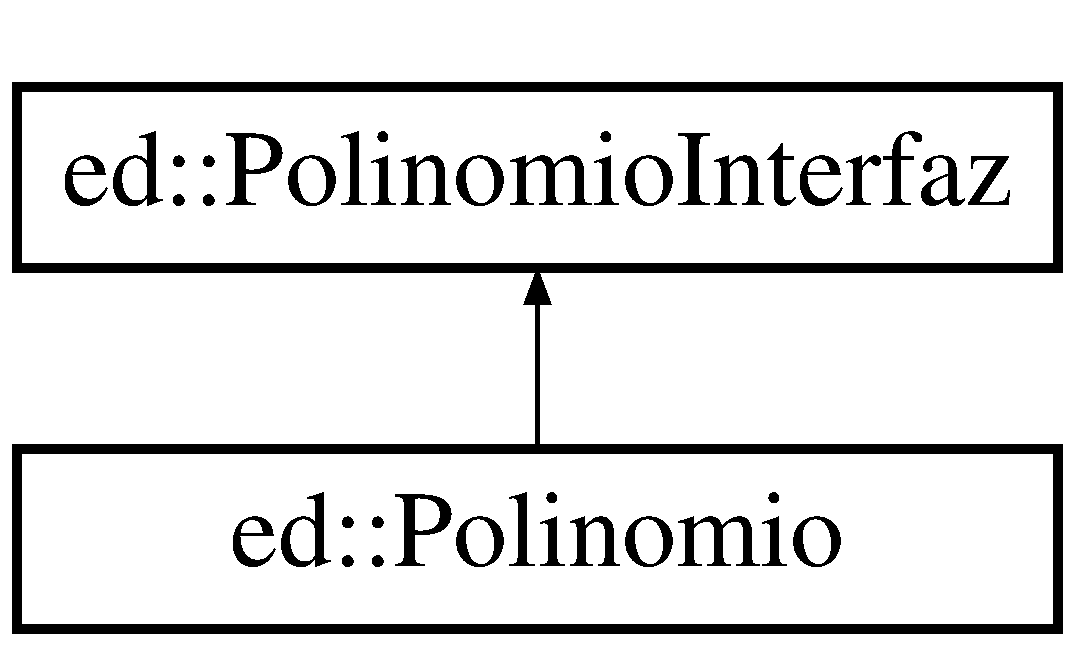
\includegraphics[height=2.000000cm]{classed_1_1Polinomio}
\end{center}
\end{figure}
\subsection*{Public Member Functions}
\begin{Indent}{\bf Atributos publicos de la clase Polinomio}\par
\begin{DoxyCompactItemize}
\item 
\hyperlink{classed_1_1Polinomio_ad2a480e2e09d0afa8f58907f5460a357}{Polinomio} (\hyperlink{classed_1_1Polinomio}{Polinomio} const \&p)
\begin{DoxyCompactList}\small\item\em Contructor que crea un polinomio a partir de otro polinomio pasado por referencia. \end{DoxyCompactList}\item 
\hyperlink{classed_1_1Polinomio_ab357d5df6da0d216f079f485937b6266}{Polinomio} (int grado=0, int terminos=0, int n=0)
\begin{DoxyCompactList}\small\item\em Contructor que crea un polinomio a partir del grado, los terminos y el numero de terminos. \end{DoxyCompactList}\item 
int \hyperlink{classed_1_1Polinomio_a6652a2361f03daf45b38a97e8b146d15}{get\-Grado} () const 
\begin{DoxyCompactList}\small\item\em Devuelve el grado del polinomio. \end{DoxyCompactList}\item 
int \hyperlink{classed_1_1Polinomio_a9c54328800c74a91e04cb22f968e7510}{get\-Terminos} () const 
\begin{DoxyCompactList}\small\item\em Devuelve el numero de terminos de un polinomio. \end{DoxyCompactList}\item 
\hyperlink{classed_1_1Monomio}{Monomio} \hyperlink{classed_1_1Polinomio_ac2b20ed929a98c449c635cc70dc82f20}{get\-Monomio} (const int i) const 
\begin{DoxyCompactList}\small\item\em Devuelve el monomio del polinomio. \end{DoxyCompactList}\item 
vector$<$ \hyperlink{classed_1_1Monomio}{Monomio} $>$ \hyperlink{classed_1_1Polinomio_a80086e21883c1108260006302135eade}{get\-Polinomio} () const 
\begin{DoxyCompactList}\small\item\em Devuelve el polinomio. \end{DoxyCompactList}\item 
void \hyperlink{classed_1_1Polinomio_acf2aa0cc5b63144eeffc603e6de0d9a3}{set\-Terminos} (const int \&terminos)
\begin{DoxyCompactList}\small\item\em Asigna un valor \char`\"{}terminos\char`\"{} al numero de terminos de un polinomio. \end{DoxyCompactList}\item 
void \hyperlink{classed_1_1Polinomio_a2387bb72b00d6d62daac94a27129d1fe}{set\-Grado} (const int \&grado)
\begin{DoxyCompactList}\small\item\em Asigna un valor \char`\"{}grado\char`\"{} al grado de un polinomio. \end{DoxyCompactList}\item 
void \hyperlink{classed_1_1Polinomio_a76864a912e2301a813c08a51b743fa26}{set\-Polinomio} (const vector$<$ \hyperlink{classed_1_1Monomio}{Monomio} $>$ \&p)
\begin{DoxyCompactList}\small\item\em Asigna un polinomio. \end{DoxyCompactList}\item 
bool \hyperlink{classed_1_1Polinomio_a1a2237c522e6e6907d119d77dcc4aca5}{test\-Polinomio} ()
\begin{DoxyCompactList}\small\item\em Comprueba si un polinomio esta vacio. \end{DoxyCompactList}\item 
\hyperlink{classed_1_1Polinomio}{Polinomio} \& \hyperlink{classed_1_1Polinomio_a324b06e0f0f9fde61625ca4a912962cc}{operator=} (\hyperlink{classed_1_1Polinomio}{Polinomio} const \&p)
\begin{DoxyCompactList}\small\item\em /name Operadores \end{DoxyCompactList}\item 
\hyperlink{classed_1_1Polinomio}{Polinomio} \hyperlink{classed_1_1Polinomio_a71d8e6f2a66622de636cac0b46609164}{operator+} (\hyperlink{classed_1_1Polinomio}{Polinomio} const \&p)
\begin{DoxyCompactList}\small\item\em Operador de suma de dos polinomios. \end{DoxyCompactList}\item 
\hyperlink{classed_1_1Polinomio}{Polinomio} \hyperlink{classed_1_1Polinomio_a547d6a82646d52dc7c950fef254c275c}{operator$\ast$} (\hyperlink{classed_1_1Polinomio}{Polinomio} const \&p)
\begin{DoxyCompactList}\small\item\em Operador de producto de dos polinomios. \end{DoxyCompactList}\item 
void \hyperlink{classed_1_1Polinomio_a7d264883d3fc0ba0b72c8c68fb55ca13}{calcular\-Grado} ()
\begin{DoxyCompactList}\small\item\em Calcula el grado de un \hyperlink{classed_1_1Polinomio}{Polinomio} y se lo asigna. \end{DoxyCompactList}\item 
void \hyperlink{classed_1_1Polinomio_ada80935d3e99914906c46592d6efdcd4}{leer\-Polinomio} ()
\begin{DoxyCompactList}\small\item\em Lee los valores de un polinomio por pantalla y se los asigna al \hyperlink{classed_1_1Polinomio}{Polinomio}. \end{DoxyCompactList}\item 
void \hyperlink{classed_1_1Polinomio_ad8c9a4ff8fd9253e42dfaa4a6ced9409}{escribir\-Polinomio} ()
\begin{DoxyCompactList}\small\item\em Escribe los valores de un polinomio por pantalla. \end{DoxyCompactList}\item 
double \hyperlink{classed_1_1Polinomio_ab2997b1a2b83727ac96fea969b69f3c7}{valor\-Polinomio} (double x)
\begin{DoxyCompactList}\small\item\em Calcula el valor de un polinomio dado un valor. \end{DoxyCompactList}\item 
vector$<$ \hyperlink{classed_1_1Monomio}{Monomio} $>$ \hyperlink{classed_1_1Polinomio_a58c42d9ddeaf9d4a3776af389809e2a9}{suma\-Vector} (vector$<$ \hyperlink{classed_1_1Monomio}{Monomio} $>$ \&p)
\begin{DoxyCompactList}\small\item\em Suma los monomios de un vector dado. \end{DoxyCompactList}\end{DoxyCompactItemize}
\end{Indent}
\subsection*{Friends}
\begin{Indent}{\bf Funciones amigas para poder acceder a la parte privada de Monomio}\par
\begin{DoxyCompactItemize}
\item 
ostream \& \hyperlink{classed_1_1Polinomio_a3f44b3043aa98d5a670c6a23cd0a6db7}{operator$<$$<$} (ostream \&stream, \hyperlink{classed_1_1Polinomio}{Polinomio} const \&p)
\begin{DoxyCompactList}\small\item\em Sobrecarga del operador de salida \char`\"{}$<$$<$\char`\"{}. \end{DoxyCompactList}\item 
istream \& \hyperlink{classed_1_1Polinomio_a11359b914d66503eb5a0a15c1983b068}{operator$>$$>$} (istream \&stream, \hyperlink{classed_1_1Polinomio}{Polinomio} \&p)
\begin{DoxyCompactList}\small\item\em Sobrecarga del operador de entrada \char`\"{}$>$$>$\char`\"{}. \end{DoxyCompactList}\end{DoxyCompactItemize}
\end{Indent}


\subsection{Detailed Description}
Definición de la clase \hyperlink{classed_1_1Polinomio}{Polinomio}. 

\subsection{Constructor \& Destructor Documentation}
\hypertarget{classed_1_1Polinomio_ad2a480e2e09d0afa8f58907f5460a357}{\index{ed\-::\-Polinomio@{ed\-::\-Polinomio}!Polinomio@{Polinomio}}
\index{Polinomio@{Polinomio}!ed::Polinomio@{ed\-::\-Polinomio}}
\subsubsection[{Polinomio}]{\setlength{\rightskip}{0pt plus 5cm}ed\-::\-Polinomio\-::\-Polinomio (
\begin{DoxyParamCaption}
\item[{{\bf Polinomio} const \&}]{p}
\end{DoxyParamCaption}
)\hspace{0.3cm}{\ttfamily [inline]}}}\label{classed_1_1Polinomio_ad2a480e2e09d0afa8f58907f5460a357}


Contructor que crea un polinomio a partir de otro polinomio pasado por referencia. 

\begin{DoxyAttention}{Attention}
Función sobrecargada 
\end{DoxyAttention}

\begin{DoxyParams}{Parameters}
{\em p} & \hyperlink{classed_1_1Polinomio}{Polinomio}, \hyperlink{classed_1_1Polinomio}{Polinomio} pasado por referencia \\
\hline
\end{DoxyParams}
\begin{DoxyPrecond}{Precondition}
Ninguna 
\end{DoxyPrecond}
\begin{DoxyPostcond}{Postcondition}
Ninguna 
\end{DoxyPostcond}
\begin{DoxySeeAlso}{See Also}
\hyperlink{classed_1_1Polinomio_a2387bb72b00d6d62daac94a27129d1fe}{set\-Grado()}, \hyperlink{classed_1_1Polinomio_acf2aa0cc5b63144eeffc603e6de0d9a3}{set\-Terminos()}, \hyperlink{classed_1_1Polinomio_a76864a912e2301a813c08a51b743fa26}{set\-Polinomio()}, \hyperlink{classed_1_1Polinomio_a6652a2361f03daf45b38a97e8b146d15}{get\-Grado()}, \hyperlink{classed_1_1Polinomio_a9c54328800c74a91e04cb22f968e7510}{get\-Terminos()}, \hyperlink{classed_1_1Polinomio_a80086e21883c1108260006302135eade}{get\-Polinomio()} 
\end{DoxySeeAlso}
\hypertarget{classed_1_1Polinomio_ab357d5df6da0d216f079f485937b6266}{\index{ed\-::\-Polinomio@{ed\-::\-Polinomio}!Polinomio@{Polinomio}}
\index{Polinomio@{Polinomio}!ed::Polinomio@{ed\-::\-Polinomio}}
\subsubsection[{Polinomio}]{\setlength{\rightskip}{0pt plus 5cm}ed\-::\-Polinomio\-::\-Polinomio (
\begin{DoxyParamCaption}
\item[{int}]{grado = {\ttfamily 0}, }
\item[{int}]{terminos = {\ttfamily 0}, }
\item[{int}]{n = {\ttfamily 0}}
\end{DoxyParamCaption}
)\hspace{0.3cm}{\ttfamily [inline]}}}\label{classed_1_1Polinomio_ab357d5df6da0d216f079f485937b6266}


Contructor que crea un polinomio a partir del grado, los terminos y el numero de terminos. 

\begin{DoxyAttention}{Attention}
Función sobrecargada 
\end{DoxyAttention}
\begin{DoxyNote}{Note}
Los parámetros tienen valores por defecto 
\end{DoxyNote}

\begin{DoxyParams}{Parameters}
{\em grado} & int, valor por defecto 0.\-0 \\
\hline
{\em terminos} & int, valor por defecto 0 \\
\hline
{\em n} & int, valor por defecto 0 \\
\hline
\end{DoxyParams}
\begin{DoxyPrecond}{Precondition}
Ninguna 
\end{DoxyPrecond}
\begin{DoxyPostcond}{Postcondition}
Ninguna 
\end{DoxyPostcond}
\begin{DoxySeeAlso}{See Also}
\hyperlink{classed_1_1Polinomio_a2387bb72b00d6d62daac94a27129d1fe}{set\-Grado()}, \hyperlink{classed_1_1Polinomio_acf2aa0cc5b63144eeffc603e6de0d9a3}{set\-Terminos()} 
\end{DoxySeeAlso}


\subsection{Member Function Documentation}
\hypertarget{classed_1_1Polinomio_a7d264883d3fc0ba0b72c8c68fb55ca13}{\index{ed\-::\-Polinomio@{ed\-::\-Polinomio}!calcular\-Grado@{calcular\-Grado}}
\index{calcular\-Grado@{calcular\-Grado}!ed::Polinomio@{ed\-::\-Polinomio}}
\subsubsection[{calcular\-Grado}]{\setlength{\rightskip}{0pt plus 5cm}void Polinomio\-::calcular\-Grado (
\begin{DoxyParamCaption}
{}
\end{DoxyParamCaption}
)}}\label{classed_1_1Polinomio_a7d264883d3fc0ba0b72c8c68fb55ca13}


Calcula el grado de un \hyperlink{classed_1_1Polinomio}{Polinomio} y se lo asigna. 

\begin{DoxyPrecond}{Precondition}
El polinomio debe existir 
\end{DoxyPrecond}
\begin{DoxyPostcond}{Postcondition}
El grado del polinomio queda modificado 
\end{DoxyPostcond}
\hypertarget{classed_1_1Polinomio_ad8c9a4ff8fd9253e42dfaa4a6ced9409}{\index{ed\-::\-Polinomio@{ed\-::\-Polinomio}!escribir\-Polinomio@{escribir\-Polinomio}}
\index{escribir\-Polinomio@{escribir\-Polinomio}!ed::Polinomio@{ed\-::\-Polinomio}}
\subsubsection[{escribir\-Polinomio}]{\setlength{\rightskip}{0pt plus 5cm}void Polinomio\-::escribir\-Polinomio (
\begin{DoxyParamCaption}
{}
\end{DoxyParamCaption}
)}}\label{classed_1_1Polinomio_ad8c9a4ff8fd9253e42dfaa4a6ced9409}


Escribe los valores de un polinomio por pantalla. 

\begin{DoxyPrecond}{Precondition}
El polinomio debe existir 
\end{DoxyPrecond}
\begin{DoxyPostcond}{Postcondition}
Ninguna 
\end{DoxyPostcond}
\hypertarget{classed_1_1Polinomio_a6652a2361f03daf45b38a97e8b146d15}{\index{ed\-::\-Polinomio@{ed\-::\-Polinomio}!get\-Grado@{get\-Grado}}
\index{get\-Grado@{get\-Grado}!ed::Polinomio@{ed\-::\-Polinomio}}
\subsubsection[{get\-Grado}]{\setlength{\rightskip}{0pt plus 5cm}int ed\-::\-Polinomio\-::get\-Grado (
\begin{DoxyParamCaption}
{}
\end{DoxyParamCaption}
) const\hspace{0.3cm}{\ttfamily [inline]}, {\ttfamily [virtual]}}}\label{classed_1_1Polinomio_a6652a2361f03daf45b38a97e8b146d15}


Devuelve el grado del polinomio. 

\begin{DoxyReturn}{Returns}
Grado de un polinomio 
\end{DoxyReturn}
\begin{DoxyPrecond}{Precondition}
El polinomio debe existir anteriormente 
\end{DoxyPrecond}
\begin{DoxyPostcond}{Postcondition}
Ninguna 
\end{DoxyPostcond}
\begin{DoxySeeAlso}{See Also}
\hyperlink{classed_1_1Polinomio_a9c54328800c74a91e04cb22f968e7510}{get\-Terminos()}, \hyperlink{classed_1_1Polinomio_ac2b20ed929a98c449c635cc70dc82f20}{get\-Monomio()}, \hyperlink{classed_1_1Polinomio_a80086e21883c1108260006302135eade}{get\-Polinomio()} 
\end{DoxySeeAlso}


Implements \hyperlink{classed_1_1PolinomioInterfaz_a7d6b7000f661d225b54486165ad4e6fc}{ed\-::\-Polinomio\-Interfaz}.

\hypertarget{classed_1_1Polinomio_ac2b20ed929a98c449c635cc70dc82f20}{\index{ed\-::\-Polinomio@{ed\-::\-Polinomio}!get\-Monomio@{get\-Monomio}}
\index{get\-Monomio@{get\-Monomio}!ed::Polinomio@{ed\-::\-Polinomio}}
\subsubsection[{get\-Monomio}]{\setlength{\rightskip}{0pt plus 5cm}{\bf Monomio} ed\-::\-Polinomio\-::get\-Monomio (
\begin{DoxyParamCaption}
\item[{const int}]{i}
\end{DoxyParamCaption}
) const\hspace{0.3cm}{\ttfamily [inline]}, {\ttfamily [virtual]}}}\label{classed_1_1Polinomio_ac2b20ed929a98c449c635cc70dc82f20}


Devuelve el monomio del polinomio. 

\begin{DoxyReturn}{Returns}
\hyperlink{classed_1_1Monomio}{Monomio} de un polinomio 
\end{DoxyReturn}

\begin{DoxyParams}{Parameters}
{\em i} & int, posicion del monomio a devolver \\
\hline
\end{DoxyParams}
\begin{DoxyPrecond}{Precondition}
El polinomio debe existir anteriormente 
\end{DoxyPrecond}
\begin{DoxyPostcond}{Postcondition}
Ninguna 
\end{DoxyPostcond}
\begin{DoxySeeAlso}{See Also}
\hyperlink{classed_1_1Polinomio_a9c54328800c74a91e04cb22f968e7510}{get\-Terminos()}, \hyperlink{classed_1_1Polinomio_a6652a2361f03daf45b38a97e8b146d15}{get\-Grado()}, \hyperlink{classed_1_1Polinomio_a80086e21883c1108260006302135eade}{get\-Polinomio()} 
\end{DoxySeeAlso}


Implements \hyperlink{classed_1_1PolinomioInterfaz_a330cdb321988ad4c9110692b8de3dac5}{ed\-::\-Polinomio\-Interfaz}.

\hypertarget{classed_1_1Polinomio_a80086e21883c1108260006302135eade}{\index{ed\-::\-Polinomio@{ed\-::\-Polinomio}!get\-Polinomio@{get\-Polinomio}}
\index{get\-Polinomio@{get\-Polinomio}!ed::Polinomio@{ed\-::\-Polinomio}}
\subsubsection[{get\-Polinomio}]{\setlength{\rightskip}{0pt plus 5cm}vector$<${\bf Monomio}$>$ ed\-::\-Polinomio\-::get\-Polinomio (
\begin{DoxyParamCaption}
{}
\end{DoxyParamCaption}
) const\hspace{0.3cm}{\ttfamily [inline]}, {\ttfamily [virtual]}}}\label{classed_1_1Polinomio_a80086e21883c1108260006302135eade}


Devuelve el polinomio. 

\begin{DoxyReturn}{Returns}
polinomio de monomios 
\end{DoxyReturn}
\begin{DoxyPrecond}{Precondition}
El monomio debe existir anteriormente 
\end{DoxyPrecond}
\begin{DoxyPostcond}{Postcondition}
Ninguna 
\end{DoxyPostcond}
\begin{DoxySeeAlso}{See Also}
\hyperlink{classed_1_1Polinomio_a9c54328800c74a91e04cb22f968e7510}{get\-Terminos()}, \hyperlink{classed_1_1Polinomio_ac2b20ed929a98c449c635cc70dc82f20}{get\-Monomio()}, \hyperlink{classed_1_1Polinomio_a6652a2361f03daf45b38a97e8b146d15}{get\-Grado()} 
\end{DoxySeeAlso}


Implements \hyperlink{classed_1_1PolinomioInterfaz_a87be8f97a3338ae8e4b71ffcb2705ca1}{ed\-::\-Polinomio\-Interfaz}.

\hypertarget{classed_1_1Polinomio_a9c54328800c74a91e04cb22f968e7510}{\index{ed\-::\-Polinomio@{ed\-::\-Polinomio}!get\-Terminos@{get\-Terminos}}
\index{get\-Terminos@{get\-Terminos}!ed::Polinomio@{ed\-::\-Polinomio}}
\subsubsection[{get\-Terminos}]{\setlength{\rightskip}{0pt plus 5cm}int ed\-::\-Polinomio\-::get\-Terminos (
\begin{DoxyParamCaption}
{}
\end{DoxyParamCaption}
) const\hspace{0.3cm}{\ttfamily [inline]}, {\ttfamily [virtual]}}}\label{classed_1_1Polinomio_a9c54328800c74a91e04cb22f968e7510}


Devuelve el numero de terminos de un polinomio. 

\begin{DoxyReturn}{Returns}
Terminos de un polinomio 
\end{DoxyReturn}
\begin{DoxyPrecond}{Precondition}
El polinomio debe existir anteriormente 
\end{DoxyPrecond}
\begin{DoxyPostcond}{Postcondition}
Ninguna 
\end{DoxyPostcond}
\begin{DoxySeeAlso}{See Also}
\hyperlink{classed_1_1Polinomio_a6652a2361f03daf45b38a97e8b146d15}{get\-Grado()}, \hyperlink{classed_1_1Polinomio_ac2b20ed929a98c449c635cc70dc82f20}{get\-Monomio()}, \hyperlink{classed_1_1Polinomio_a80086e21883c1108260006302135eade}{get\-Polinomio()} 
\end{DoxySeeAlso}


Implements \hyperlink{classed_1_1PolinomioInterfaz_ad4d96c242782ff75116e0c1c1d37b680}{ed\-::\-Polinomio\-Interfaz}.

\hypertarget{classed_1_1Polinomio_ada80935d3e99914906c46592d6efdcd4}{\index{ed\-::\-Polinomio@{ed\-::\-Polinomio}!leer\-Polinomio@{leer\-Polinomio}}
\index{leer\-Polinomio@{leer\-Polinomio}!ed::Polinomio@{ed\-::\-Polinomio}}
\subsubsection[{leer\-Polinomio}]{\setlength{\rightskip}{0pt plus 5cm}void Polinomio\-::leer\-Polinomio (
\begin{DoxyParamCaption}
{}
\end{DoxyParamCaption}
)}}\label{classed_1_1Polinomio_ada80935d3e99914906c46592d6efdcd4}


Lee los valores de un polinomio por pantalla y se los asigna al \hyperlink{classed_1_1Polinomio}{Polinomio}. 

\begin{DoxyPrecond}{Precondition}
El polinomio debe existir 
\end{DoxyPrecond}
\begin{DoxyPostcond}{Postcondition}
El polinomio es modificado 
\end{DoxyPostcond}
\hypertarget{classed_1_1Polinomio_a547d6a82646d52dc7c950fef254c275c}{\index{ed\-::\-Polinomio@{ed\-::\-Polinomio}!operator$\ast$@{operator$\ast$}}
\index{operator$\ast$@{operator$\ast$}!ed::Polinomio@{ed\-::\-Polinomio}}
\subsubsection[{operator$\ast$}]{\setlength{\rightskip}{0pt plus 5cm}{\bf Polinomio} ed\-::\-Polinomio\-::operator$\ast$ (
\begin{DoxyParamCaption}
\item[{{\bf Polinomio} const \&}]{p}
\end{DoxyParamCaption}
)\hspace{0.3cm}{\ttfamily [inline]}}}\label{classed_1_1Polinomio_a547d6a82646d52dc7c950fef254c275c}


Operador de producto de dos polinomios. 

\begin{DoxyAttention}{Attention}
Se sobrecarga el operador de suma 
\end{DoxyAttention}

\begin{DoxyParams}{Parameters}
{\em p} & \hyperlink{classed_1_1Polinomio}{Polinomio} pasado por referencia constante \\
\hline
\end{DoxyParams}
\begin{DoxyReturn}{Returns}
Producto de dos polinomios 
\end{DoxyReturn}
\begin{DoxyPrecond}{Precondition}
El polinomio debe existir 
\end{DoxyPrecond}
\begin{DoxyPostcond}{Postcondition}
Ninguna 
\end{DoxyPostcond}
\begin{DoxySeeAlso}{See Also}
\hyperlink{classed_1_1Polinomio_a2387bb72b00d6d62daac94a27129d1fe}{set\-Grado()}, \hyperlink{classed_1_1Polinomio_acf2aa0cc5b63144eeffc603e6de0d9a3}{set\-Terminos()}, \hyperlink{classed_1_1Polinomio_a76864a912e2301a813c08a51b743fa26}{set\-Polinomio()}, \hyperlink{classed_1_1Polinomio_a6652a2361f03daf45b38a97e8b146d15}{get\-Grado()}, \hyperlink{classed_1_1Polinomio_a9c54328800c74a91e04cb22f968e7510}{get\-Terminos()}, \hyperlink{classed_1_1Polinomio_a80086e21883c1108260006302135eade}{get\-Polinomio()} 
\end{DoxySeeAlso}
\hypertarget{classed_1_1Polinomio_a71d8e6f2a66622de636cac0b46609164}{\index{ed\-::\-Polinomio@{ed\-::\-Polinomio}!operator+@{operator+}}
\index{operator+@{operator+}!ed::Polinomio@{ed\-::\-Polinomio}}
\subsubsection[{operator+}]{\setlength{\rightskip}{0pt plus 5cm}{\bf Polinomio} ed\-::\-Polinomio\-::operator+ (
\begin{DoxyParamCaption}
\item[{{\bf Polinomio} const \&}]{p}
\end{DoxyParamCaption}
)\hspace{0.3cm}{\ttfamily [inline]}}}\label{classed_1_1Polinomio_a71d8e6f2a66622de636cac0b46609164}


Operador de suma de dos polinomios. 

\begin{DoxyAttention}{Attention}
Se sobrecarga el operador de suma 
\end{DoxyAttention}

\begin{DoxyParams}{Parameters}
{\em p} & \hyperlink{classed_1_1Polinomio}{Polinomio} pasado por referencia constante \\
\hline
\end{DoxyParams}
\begin{DoxyReturn}{Returns}
Suma de dos polinomios 
\end{DoxyReturn}
\begin{DoxyPrecond}{Precondition}
El polinomio debe existir 
\end{DoxyPrecond}
\begin{DoxyPostcond}{Postcondition}
Ninguna 
\end{DoxyPostcond}
\begin{DoxySeeAlso}{See Also}
\hyperlink{classed_1_1Polinomio_a2387bb72b00d6d62daac94a27129d1fe}{set\-Grado()}, \hyperlink{classed_1_1Polinomio_acf2aa0cc5b63144eeffc603e6de0d9a3}{set\-Terminos()}, \hyperlink{classed_1_1Polinomio_a76864a912e2301a813c08a51b743fa26}{set\-Polinomio()}, \hyperlink{classed_1_1Polinomio_a6652a2361f03daf45b38a97e8b146d15}{get\-Grado()}, \hyperlink{classed_1_1Polinomio_a9c54328800c74a91e04cb22f968e7510}{get\-Terminos()}, \hyperlink{classed_1_1Polinomio_a80086e21883c1108260006302135eade}{get\-Polinomio()} 
\end{DoxySeeAlso}
\hypertarget{classed_1_1Polinomio_a324b06e0f0f9fde61625ca4a912962cc}{\index{ed\-::\-Polinomio@{ed\-::\-Polinomio}!operator=@{operator=}}
\index{operator=@{operator=}!ed::Polinomio@{ed\-::\-Polinomio}}
\subsubsection[{operator=}]{\setlength{\rightskip}{0pt plus 5cm}{\bf Polinomio}\& ed\-::\-Polinomio\-::operator= (
\begin{DoxyParamCaption}
\item[{{\bf Polinomio} const \&}]{p}
\end{DoxyParamCaption}
)\hspace{0.3cm}{\ttfamily [inline]}}}\label{classed_1_1Polinomio_a324b06e0f0f9fde61625ca4a912962cc}


/name Operadores 

Operador de copia de un polinomio en otro \begin{DoxyAttention}{Attention}
Se sobrecarga el operador de asignacion 
\end{DoxyAttention}

\begin{DoxyParams}{Parameters}
{\em p} & \hyperlink{classed_1_1Polinomio}{Polinomio} pasado por referencia constante \\
\hline
\end{DoxyParams}
\begin{DoxyPrecond}{Precondition}
El polinomio debe existir 
\end{DoxyPrecond}
\begin{DoxyPostcond}{Postcondition}
Ninguna 
\end{DoxyPostcond}
\begin{DoxySeeAlso}{See Also}
\hyperlink{classed_1_1Polinomio_a2387bb72b00d6d62daac94a27129d1fe}{set\-Grado()}, \hyperlink{classed_1_1Polinomio_acf2aa0cc5b63144eeffc603e6de0d9a3}{set\-Terminos()}, \hyperlink{classed_1_1Polinomio_a76864a912e2301a813c08a51b743fa26}{set\-Polinomio()}, \hyperlink{classed_1_1Polinomio_a6652a2361f03daf45b38a97e8b146d15}{get\-Grado()}, \hyperlink{classed_1_1Polinomio_a9c54328800c74a91e04cb22f968e7510}{get\-Terminos()}, \hyperlink{classed_1_1Polinomio_a80086e21883c1108260006302135eade}{get\-Polinomio()} 
\end{DoxySeeAlso}
\hypertarget{classed_1_1Polinomio_a2387bb72b00d6d62daac94a27129d1fe}{\index{ed\-::\-Polinomio@{ed\-::\-Polinomio}!set\-Grado@{set\-Grado}}
\index{set\-Grado@{set\-Grado}!ed::Polinomio@{ed\-::\-Polinomio}}
\subsubsection[{set\-Grado}]{\setlength{\rightskip}{0pt plus 5cm}void ed\-::\-Polinomio\-::set\-Grado (
\begin{DoxyParamCaption}
\item[{const int \&}]{grado}
\end{DoxyParamCaption}
)\hspace{0.3cm}{\ttfamily [inline]}, {\ttfamily [virtual]}}}\label{classed_1_1Polinomio_a2387bb72b00d6d62daac94a27129d1fe}


Asigna un valor \char`\"{}grado\char`\"{} al grado de un polinomio. 


\begin{DoxyParams}{Parameters}
{\em grado} & int pasado por referencia constante \\
\hline
\end{DoxyParams}
\begin{DoxyPrecond}{Precondition}
El polinomio debe existir 
\end{DoxyPrecond}
\begin{DoxyPostcond}{Postcondition}
Ninguna 
\end{DoxyPostcond}
\begin{DoxySeeAlso}{See Also}
\hyperlink{classed_1_1Polinomio_acf2aa0cc5b63144eeffc603e6de0d9a3}{set\-Terminos()}, \hyperlink{classed_1_1Polinomio_a76864a912e2301a813c08a51b743fa26}{set\-Polinomio()} 
\end{DoxySeeAlso}


Implements \hyperlink{classed_1_1PolinomioInterfaz_a826853f0089f5939ebcd31aa18d6a735}{ed\-::\-Polinomio\-Interfaz}.

\hypertarget{classed_1_1Polinomio_a76864a912e2301a813c08a51b743fa26}{\index{ed\-::\-Polinomio@{ed\-::\-Polinomio}!set\-Polinomio@{set\-Polinomio}}
\index{set\-Polinomio@{set\-Polinomio}!ed::Polinomio@{ed\-::\-Polinomio}}
\subsubsection[{set\-Polinomio}]{\setlength{\rightskip}{0pt plus 5cm}void ed\-::\-Polinomio\-::set\-Polinomio (
\begin{DoxyParamCaption}
\item[{const vector$<$ {\bf Monomio} $>$ \&}]{p}
\end{DoxyParamCaption}
)\hspace{0.3cm}{\ttfamily [inline]}, {\ttfamily [virtual]}}}\label{classed_1_1Polinomio_a76864a912e2301a813c08a51b743fa26}


Asigna un polinomio. 


\begin{DoxyParams}{Parameters}
{\em p} & vector \hyperlink{classed_1_1Monomio}{Monomio} pasado por referencia constante \\
\hline
\end{DoxyParams}
\begin{DoxyPrecond}{Precondition}
El polinomio debe existir 
\end{DoxyPrecond}
\begin{DoxyPostcond}{Postcondition}
Ninguna 
\end{DoxyPostcond}
\begin{DoxySeeAlso}{See Also}
\hyperlink{classed_1_1Polinomio_a2387bb72b00d6d62daac94a27129d1fe}{set\-Grado()}, set\-Terminos(1) 
\end{DoxySeeAlso}


Implements \hyperlink{classed_1_1PolinomioInterfaz_a7c975f5f483e4eb769e27503fd1fe77d}{ed\-::\-Polinomio\-Interfaz}.

\hypertarget{classed_1_1Polinomio_acf2aa0cc5b63144eeffc603e6de0d9a3}{\index{ed\-::\-Polinomio@{ed\-::\-Polinomio}!set\-Terminos@{set\-Terminos}}
\index{set\-Terminos@{set\-Terminos}!ed::Polinomio@{ed\-::\-Polinomio}}
\subsubsection[{set\-Terminos}]{\setlength{\rightskip}{0pt plus 5cm}void ed\-::\-Polinomio\-::set\-Terminos (
\begin{DoxyParamCaption}
\item[{const int \&}]{terminos}
\end{DoxyParamCaption}
)\hspace{0.3cm}{\ttfamily [inline]}, {\ttfamily [virtual]}}}\label{classed_1_1Polinomio_acf2aa0cc5b63144eeffc603e6de0d9a3}


Asigna un valor \char`\"{}terminos\char`\"{} al numero de terminos de un polinomio. 


\begin{DoxyParams}{Parameters}
{\em terminos} & int pasado por referencia constante \\
\hline
\end{DoxyParams}
\begin{DoxyPrecond}{Precondition}
El polinomio debe existir 
\end{DoxyPrecond}
\begin{DoxyPostcond}{Postcondition}
Ninguna 
\end{DoxyPostcond}
\begin{DoxySeeAlso}{See Also}
\hyperlink{classed_1_1Polinomio_a2387bb72b00d6d62daac94a27129d1fe}{set\-Grado()}, \hyperlink{classed_1_1Polinomio_a76864a912e2301a813c08a51b743fa26}{set\-Polinomio()} 
\end{DoxySeeAlso}


Implements \hyperlink{classed_1_1PolinomioInterfaz_a7559c60d1b56617ae28b60f359b67fbe}{ed\-::\-Polinomio\-Interfaz}.

\hypertarget{classed_1_1Polinomio_a58c42d9ddeaf9d4a3776af389809e2a9}{\index{ed\-::\-Polinomio@{ed\-::\-Polinomio}!suma\-Vector@{suma\-Vector}}
\index{suma\-Vector@{suma\-Vector}!ed::Polinomio@{ed\-::\-Polinomio}}
\subsubsection[{suma\-Vector}]{\setlength{\rightskip}{0pt plus 5cm}vector$<$ {\bf Monomio} $>$ Polinomio\-::suma\-Vector (
\begin{DoxyParamCaption}
\item[{vector$<$ {\bf Monomio} $>$ \&}]{p}
\end{DoxyParamCaption}
)}}\label{classed_1_1Polinomio_a58c42d9ddeaf9d4a3776af389809e2a9}


Suma los monomios de un vector dado. 


\begin{DoxyParams}{Parameters}
{\em p} & vector \hyperlink{classed_1_1Monomio}{Monomio}, vector que se debe sumar \\
\hline
\end{DoxyParams}
\begin{DoxyReturn}{Returns}
\hyperlink{classed_1_1Polinomio}{Polinomio} sumado 
\end{DoxyReturn}
\begin{DoxyPrecond}{Precondition}
El vector debe existir 
\end{DoxyPrecond}
\begin{DoxyPostcond}{Postcondition}
Ninguna 
\end{DoxyPostcond}
\hypertarget{classed_1_1Polinomio_a1a2237c522e6e6907d119d77dcc4aca5}{\index{ed\-::\-Polinomio@{ed\-::\-Polinomio}!test\-Polinomio@{test\-Polinomio}}
\index{test\-Polinomio@{test\-Polinomio}!ed::Polinomio@{ed\-::\-Polinomio}}
\subsubsection[{test\-Polinomio}]{\setlength{\rightskip}{0pt plus 5cm}bool ed\-::\-Polinomio\-::test\-Polinomio (
\begin{DoxyParamCaption}
{}
\end{DoxyParamCaption}
)\hspace{0.3cm}{\ttfamily [inline]}, {\ttfamily [virtual]}}}\label{classed_1_1Polinomio_a1a2237c522e6e6907d119d77dcc4aca5}


Comprueba si un polinomio esta vacio. 

\begin{DoxyPrecond}{Precondition}
El polinomio debe existir 
\end{DoxyPrecond}
\begin{DoxyPostcond}{Postcondition}
Ninguna 
\end{DoxyPostcond}


Implements \hyperlink{classed_1_1PolinomioInterfaz_aa6972b28495fd863d484069573bf7210}{ed\-::\-Polinomio\-Interfaz}.

\hypertarget{classed_1_1Polinomio_ab2997b1a2b83727ac96fea969b69f3c7}{\index{ed\-::\-Polinomio@{ed\-::\-Polinomio}!valor\-Polinomio@{valor\-Polinomio}}
\index{valor\-Polinomio@{valor\-Polinomio}!ed::Polinomio@{ed\-::\-Polinomio}}
\subsubsection[{valor\-Polinomio}]{\setlength{\rightskip}{0pt plus 5cm}double Polinomio\-::valor\-Polinomio (
\begin{DoxyParamCaption}
\item[{double}]{x}
\end{DoxyParamCaption}
)}}\label{classed_1_1Polinomio_ab2997b1a2b83727ac96fea969b69f3c7}


Calcula el valor de un polinomio dado un valor. 


\begin{DoxyParams}{Parameters}
{\em x} & double, valor para calcular el polinomio \\
\hline
\end{DoxyParams}
\begin{DoxyReturn}{Returns}
Valor del polinomio 
\end{DoxyReturn}
\begin{DoxyPrecond}{Precondition}
El polinomio debe existir 
\end{DoxyPrecond}
\begin{DoxyPostcond}{Postcondition}
Ninguna 
\end{DoxyPostcond}


\subsection{Friends And Related Function Documentation}
\hypertarget{classed_1_1Polinomio_a3f44b3043aa98d5a670c6a23cd0a6db7}{\index{ed\-::\-Polinomio@{ed\-::\-Polinomio}!operator$<$$<$@{operator$<$$<$}}
\index{operator$<$$<$@{operator$<$$<$}!ed::Polinomio@{ed\-::\-Polinomio}}
\subsubsection[{operator$<$$<$}]{\setlength{\rightskip}{0pt plus 5cm}ostream\& operator$<$$<$ (
\begin{DoxyParamCaption}
\item[{ostream \&}]{stream, }
\item[{{\bf Polinomio} const \&}]{p}
\end{DoxyParamCaption}
)\hspace{0.3cm}{\ttfamily [friend]}}}\label{classed_1_1Polinomio_a3f44b3043aa98d5a670c6a23cd0a6db7}


Sobrecarga del operador de salida \char`\"{}$<$$<$\char`\"{}. 

\begin{DoxyAttention}{Attention}
Funcion amiga de la clase \hyperlink{classed_1_1Polinomio}{Polinomio} 
\end{DoxyAttention}

\begin{DoxyParams}{Parameters}
{\em stream} & ostream, flujo de salida \\
\hline
{\em p} & \hyperlink{classed_1_1Polinomio}{Polinomio}, pasado por referencia constante \\
\hline
\end{DoxyParams}
\begin{DoxyPrecond}{Precondition}
El \hyperlink{classed_1_1Polinomio}{Polinomio} debe existir 
\end{DoxyPrecond}
\begin{DoxyPostcond}{Postcondition}
Se escribe por pantalla el \hyperlink{classed_1_1Polinomio}{Polinomio} 
\end{DoxyPostcond}
\begin{DoxySeeAlso}{See Also}
operator $>$$>$ 
\end{DoxySeeAlso}
\hypertarget{classed_1_1Polinomio_a11359b914d66503eb5a0a15c1983b068}{\index{ed\-::\-Polinomio@{ed\-::\-Polinomio}!operator$>$$>$@{operator$>$$>$}}
\index{operator$>$$>$@{operator$>$$>$}!ed::Polinomio@{ed\-::\-Polinomio}}
\subsubsection[{operator$>$$>$}]{\setlength{\rightskip}{0pt plus 5cm}istream\& operator$>$$>$ (
\begin{DoxyParamCaption}
\item[{istream \&}]{stream, }
\item[{{\bf Polinomio} \&}]{p}
\end{DoxyParamCaption}
)\hspace{0.3cm}{\ttfamily [friend]}}}\label{classed_1_1Polinomio_a11359b914d66503eb5a0a15c1983b068}


Sobrecarga del operador de entrada \char`\"{}$>$$>$\char`\"{}. 

\begin{DoxyAttention}{Attention}
Funcion amiga de la clase \hyperlink{classed_1_1Polinomio}{Polinomio} 
\end{DoxyAttention}

\begin{DoxyParams}{Parameters}
{\em stream} & istream, flujo de entrada \\
\hline
{\em p} & \hyperlink{classed_1_1Polinomio}{Polinomio}, pasado por referencia \\
\hline
\end{DoxyParams}
\begin{DoxyPrecond}{Precondition}
El \hyperlink{classed_1_1Polinomio}{Polinomio} debe existir 
\end{DoxyPrecond}
\begin{DoxyPostcond}{Postcondition}
Se le asignan los valores al polinomio 
\end{DoxyPostcond}
\begin{DoxySeeAlso}{See Also}
operator $<$$<$ 
\end{DoxySeeAlso}


The documentation for this class was generated from the following files\-:\begin{DoxyCompactItemize}
\item 
polinomio.\-hpp\item 
polinomio.\-cpp\end{DoxyCompactItemize}

\hypertarget{classed_1_1PolinomioInterfaz}{\section{ed\-:\-:Polinomio\-Interfaz Class Reference}
\label{classed_1_1PolinomioInterfaz}\index{ed\-::\-Polinomio\-Interfaz@{ed\-::\-Polinomio\-Interfaz}}
}


Definición de la clase \hyperlink{classed_1_1PolinomioInterfaz}{Polinomio\-Interfaz}.  




{\ttfamily \#include $<$polinomio\-Interfaz.\-hpp$>$}

Inheritance diagram for ed\-:\-:Polinomio\-Interfaz\-:\begin{figure}[H]
\begin{center}
\leavevmode
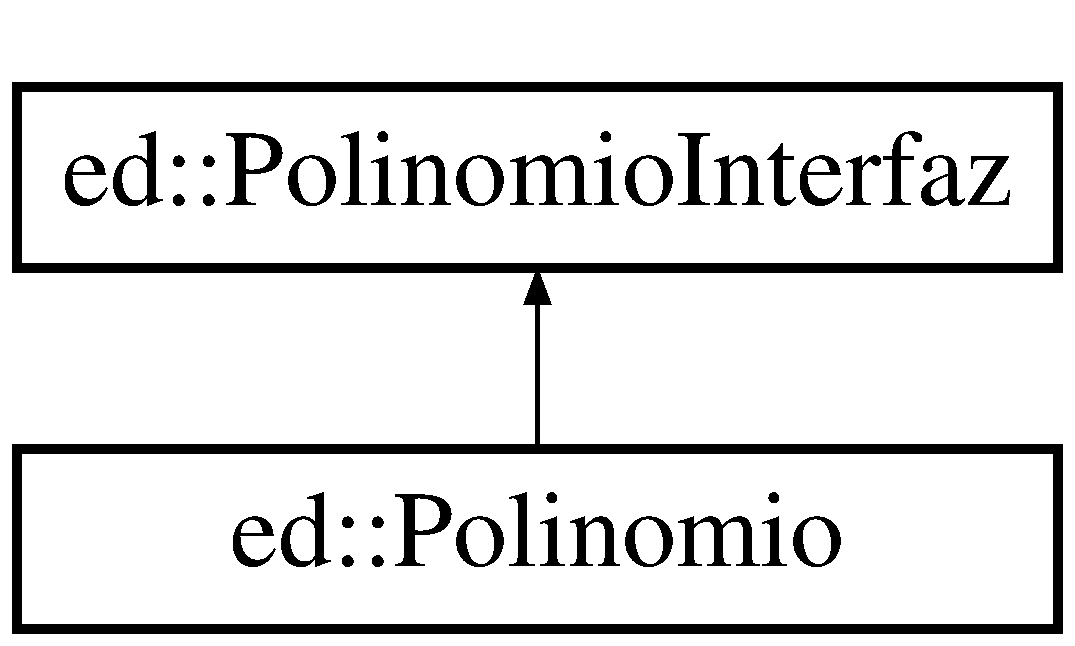
\includegraphics[height=2.000000cm]{classed_1_1PolinomioInterfaz}
\end{center}
\end{figure}
\subsection*{Public Member Functions}
\begin{Indent}{\bf Atributos publicos de la clase Polinomio}\par
\begin{DoxyCompactItemize}
\item 
virtual int \hyperlink{classed_1_1PolinomioInterfaz_ad4d96c242782ff75116e0c1c1d37b680}{get\-Terminos} () const =0
\begin{DoxyCompactList}\small\item\em Devuelve el numero de terminos de un polinomio. \end{DoxyCompactList}\item 
virtual int \hyperlink{classed_1_1PolinomioInterfaz_a7d6b7000f661d225b54486165ad4e6fc}{get\-Grado} () const =0
\begin{DoxyCompactList}\small\item\em Devuelve el grado del polinomio. \end{DoxyCompactList}\item 
virtual \hyperlink{classed_1_1Monomio}{Monomio} \hyperlink{classed_1_1PolinomioInterfaz_a330cdb321988ad4c9110692b8de3dac5}{get\-Monomio} (const int i) const =0
\begin{DoxyCompactList}\small\item\em Devuelve el monomio del polinomio. \end{DoxyCompactList}\item 
virtual vector$<$ \hyperlink{classed_1_1Monomio}{Monomio} $>$ \hyperlink{classed_1_1PolinomioInterfaz_a87be8f97a3338ae8e4b71ffcb2705ca1}{get\-Polinomio} () const =0
\begin{DoxyCompactList}\small\item\em Devuelve el polinomio. \end{DoxyCompactList}\item 
virtual void \hyperlink{classed_1_1PolinomioInterfaz_a7559c60d1b56617ae28b60f359b67fbe}{set\-Terminos} (const int \&terminos)=0
\begin{DoxyCompactList}\small\item\em Asigna un valor \char`\"{}terminos\char`\"{} al numero de terminos de un polinomio. \end{DoxyCompactList}\item 
virtual void \hyperlink{classed_1_1PolinomioInterfaz_a826853f0089f5939ebcd31aa18d6a735}{set\-Grado} (const int \&grado)=0
\begin{DoxyCompactList}\small\item\em Asigna un valor \char`\"{}grado\char`\"{} al grado de un polinomio. \end{DoxyCompactList}\item 
virtual void \hyperlink{classed_1_1PolinomioInterfaz_a7c975f5f483e4eb769e27503fd1fe77d}{set\-Polinomio} (const vector$<$ \hyperlink{classed_1_1Monomio}{Monomio} $>$ \&p)=0
\begin{DoxyCompactList}\small\item\em Asigna un polinomio. \end{DoxyCompactList}\item 
virtual bool \hyperlink{classed_1_1PolinomioInterfaz_aa6972b28495fd863d484069573bf7210}{test\-Polinomio} ()=0
\begin{DoxyCompactList}\small\item\em Comprueba si un polinomio esta vacio. \end{DoxyCompactList}\end{DoxyCompactItemize}
\end{Indent}


\subsection{Detailed Description}
Definición de la clase \hyperlink{classed_1_1PolinomioInterfaz}{Polinomio\-Interfaz}. 

\subsection{Member Function Documentation}
\hypertarget{classed_1_1PolinomioInterfaz_a7d6b7000f661d225b54486165ad4e6fc}{\index{ed\-::\-Polinomio\-Interfaz@{ed\-::\-Polinomio\-Interfaz}!get\-Grado@{get\-Grado}}
\index{get\-Grado@{get\-Grado}!ed::PolinomioInterfaz@{ed\-::\-Polinomio\-Interfaz}}
\subsubsection[{get\-Grado}]{\setlength{\rightskip}{0pt plus 5cm}virtual int ed\-::\-Polinomio\-Interfaz\-::get\-Grado (
\begin{DoxyParamCaption}
{}
\end{DoxyParamCaption}
) const\hspace{0.3cm}{\ttfamily [pure virtual]}}}\label{classed_1_1PolinomioInterfaz_a7d6b7000f661d225b54486165ad4e6fc}


Devuelve el grado del polinomio. 

\begin{DoxyReturn}{Returns}
Grado de un polinomio 
\end{DoxyReturn}
\begin{DoxyPrecond}{Precondition}
El polinomio debe existir anteriormente 
\end{DoxyPrecond}
\begin{DoxyPostcond}{Postcondition}
Ninguna 
\end{DoxyPostcond}
\begin{DoxySeeAlso}{See Also}
\hyperlink{classed_1_1PolinomioInterfaz_ad4d96c242782ff75116e0c1c1d37b680}{get\-Terminos()}, \hyperlink{classed_1_1PolinomioInterfaz_a330cdb321988ad4c9110692b8de3dac5}{get\-Monomio()}, \hyperlink{classed_1_1PolinomioInterfaz_a87be8f97a3338ae8e4b71ffcb2705ca1}{get\-Polinomio()} 
\end{DoxySeeAlso}


Implemented in \hyperlink{classed_1_1Polinomio_a6652a2361f03daf45b38a97e8b146d15}{ed\-::\-Polinomio}.

\hypertarget{classed_1_1PolinomioInterfaz_a330cdb321988ad4c9110692b8de3dac5}{\index{ed\-::\-Polinomio\-Interfaz@{ed\-::\-Polinomio\-Interfaz}!get\-Monomio@{get\-Monomio}}
\index{get\-Monomio@{get\-Monomio}!ed::PolinomioInterfaz@{ed\-::\-Polinomio\-Interfaz}}
\subsubsection[{get\-Monomio}]{\setlength{\rightskip}{0pt plus 5cm}virtual {\bf Monomio} ed\-::\-Polinomio\-Interfaz\-::get\-Monomio (
\begin{DoxyParamCaption}
\item[{const int}]{i}
\end{DoxyParamCaption}
) const\hspace{0.3cm}{\ttfamily [pure virtual]}}}\label{classed_1_1PolinomioInterfaz_a330cdb321988ad4c9110692b8de3dac5}


Devuelve el monomio del polinomio. 

\begin{DoxyReturn}{Returns}
\hyperlink{classed_1_1Monomio}{Monomio} de un polinomio 
\end{DoxyReturn}

\begin{DoxyParams}{Parameters}
{\em i} & int, posicion del monomio a devolver \\
\hline
\end{DoxyParams}
\begin{DoxyPrecond}{Precondition}
El polinomio debe existir anteriormente 
\end{DoxyPrecond}
\begin{DoxyPostcond}{Postcondition}
Ninguna 
\end{DoxyPostcond}
\begin{DoxySeeAlso}{See Also}
\hyperlink{classed_1_1PolinomioInterfaz_ad4d96c242782ff75116e0c1c1d37b680}{get\-Terminos()}, \hyperlink{classed_1_1PolinomioInterfaz_a7d6b7000f661d225b54486165ad4e6fc}{get\-Grado()}, \hyperlink{classed_1_1PolinomioInterfaz_a87be8f97a3338ae8e4b71ffcb2705ca1}{get\-Polinomio()} 
\end{DoxySeeAlso}


Implemented in \hyperlink{classed_1_1Polinomio_ac2b20ed929a98c449c635cc70dc82f20}{ed\-::\-Polinomio}.

\hypertarget{classed_1_1PolinomioInterfaz_a87be8f97a3338ae8e4b71ffcb2705ca1}{\index{ed\-::\-Polinomio\-Interfaz@{ed\-::\-Polinomio\-Interfaz}!get\-Polinomio@{get\-Polinomio}}
\index{get\-Polinomio@{get\-Polinomio}!ed::PolinomioInterfaz@{ed\-::\-Polinomio\-Interfaz}}
\subsubsection[{get\-Polinomio}]{\setlength{\rightskip}{0pt plus 5cm}virtual vector$<${\bf Monomio}$>$ ed\-::\-Polinomio\-Interfaz\-::get\-Polinomio (
\begin{DoxyParamCaption}
{}
\end{DoxyParamCaption}
) const\hspace{0.3cm}{\ttfamily [pure virtual]}}}\label{classed_1_1PolinomioInterfaz_a87be8f97a3338ae8e4b71ffcb2705ca1}


Devuelve el polinomio. 

\begin{DoxyReturn}{Returns}
polinomio de monomios 
\end{DoxyReturn}
\begin{DoxyPrecond}{Precondition}
El monomio debe existir anteriormente 
\end{DoxyPrecond}
\begin{DoxyPostcond}{Postcondition}
Ninguna 
\end{DoxyPostcond}
\begin{DoxySeeAlso}{See Also}
\hyperlink{classed_1_1PolinomioInterfaz_ad4d96c242782ff75116e0c1c1d37b680}{get\-Terminos()}, \hyperlink{classed_1_1PolinomioInterfaz_a330cdb321988ad4c9110692b8de3dac5}{get\-Monomio()}, \hyperlink{classed_1_1PolinomioInterfaz_a7d6b7000f661d225b54486165ad4e6fc}{get\-Grado()} 
\end{DoxySeeAlso}


Implemented in \hyperlink{classed_1_1Polinomio_a80086e21883c1108260006302135eade}{ed\-::\-Polinomio}.

\hypertarget{classed_1_1PolinomioInterfaz_ad4d96c242782ff75116e0c1c1d37b680}{\index{ed\-::\-Polinomio\-Interfaz@{ed\-::\-Polinomio\-Interfaz}!get\-Terminos@{get\-Terminos}}
\index{get\-Terminos@{get\-Terminos}!ed::PolinomioInterfaz@{ed\-::\-Polinomio\-Interfaz}}
\subsubsection[{get\-Terminos}]{\setlength{\rightskip}{0pt plus 5cm}virtual int ed\-::\-Polinomio\-Interfaz\-::get\-Terminos (
\begin{DoxyParamCaption}
{}
\end{DoxyParamCaption}
) const\hspace{0.3cm}{\ttfamily [pure virtual]}}}\label{classed_1_1PolinomioInterfaz_ad4d96c242782ff75116e0c1c1d37b680}


Devuelve el numero de terminos de un polinomio. 

\begin{DoxyReturn}{Returns}
Terminos de un polinomio 
\end{DoxyReturn}
\begin{DoxyPrecond}{Precondition}
El polinomio debe existir anteriormente 
\end{DoxyPrecond}
\begin{DoxyPostcond}{Postcondition}
Ninguna 
\end{DoxyPostcond}
\begin{DoxySeeAlso}{See Also}
\hyperlink{classed_1_1PolinomioInterfaz_a7d6b7000f661d225b54486165ad4e6fc}{get\-Grado()}, \hyperlink{classed_1_1PolinomioInterfaz_a330cdb321988ad4c9110692b8de3dac5}{get\-Monomio()}, \hyperlink{classed_1_1PolinomioInterfaz_a87be8f97a3338ae8e4b71ffcb2705ca1}{get\-Polinomio()} 
\end{DoxySeeAlso}


Implemented in \hyperlink{classed_1_1Polinomio_a9c54328800c74a91e04cb22f968e7510}{ed\-::\-Polinomio}.

\hypertarget{classed_1_1PolinomioInterfaz_a826853f0089f5939ebcd31aa18d6a735}{\index{ed\-::\-Polinomio\-Interfaz@{ed\-::\-Polinomio\-Interfaz}!set\-Grado@{set\-Grado}}
\index{set\-Grado@{set\-Grado}!ed::PolinomioInterfaz@{ed\-::\-Polinomio\-Interfaz}}
\subsubsection[{set\-Grado}]{\setlength{\rightskip}{0pt plus 5cm}virtual void ed\-::\-Polinomio\-Interfaz\-::set\-Grado (
\begin{DoxyParamCaption}
\item[{const int \&}]{grado}
\end{DoxyParamCaption}
)\hspace{0.3cm}{\ttfamily [pure virtual]}}}\label{classed_1_1PolinomioInterfaz_a826853f0089f5939ebcd31aa18d6a735}


Asigna un valor \char`\"{}grado\char`\"{} al grado de un polinomio. 


\begin{DoxyParams}{Parameters}
{\em grado} & int pasado por referencia constante \\
\hline
\end{DoxyParams}
\begin{DoxyPrecond}{Precondition}
El polinomio debe existir 
\end{DoxyPrecond}
\begin{DoxyPostcond}{Postcondition}
Ninguna 
\end{DoxyPostcond}
\begin{DoxySeeAlso}{See Also}
\hyperlink{classed_1_1PolinomioInterfaz_a7559c60d1b56617ae28b60f359b67fbe}{set\-Terminos()}, \hyperlink{classed_1_1PolinomioInterfaz_a7c975f5f483e4eb769e27503fd1fe77d}{set\-Polinomio()} 
\end{DoxySeeAlso}


Implemented in \hyperlink{classed_1_1Polinomio_a2387bb72b00d6d62daac94a27129d1fe}{ed\-::\-Polinomio}.

\hypertarget{classed_1_1PolinomioInterfaz_a7c975f5f483e4eb769e27503fd1fe77d}{\index{ed\-::\-Polinomio\-Interfaz@{ed\-::\-Polinomio\-Interfaz}!set\-Polinomio@{set\-Polinomio}}
\index{set\-Polinomio@{set\-Polinomio}!ed::PolinomioInterfaz@{ed\-::\-Polinomio\-Interfaz}}
\subsubsection[{set\-Polinomio}]{\setlength{\rightskip}{0pt plus 5cm}virtual void ed\-::\-Polinomio\-Interfaz\-::set\-Polinomio (
\begin{DoxyParamCaption}
\item[{const vector$<$ {\bf Monomio} $>$ \&}]{p}
\end{DoxyParamCaption}
)\hspace{0.3cm}{\ttfamily [pure virtual]}}}\label{classed_1_1PolinomioInterfaz_a7c975f5f483e4eb769e27503fd1fe77d}


Asigna un polinomio. 


\begin{DoxyParams}{Parameters}
{\em p} & vector \hyperlink{classed_1_1Monomio}{Monomio} pasado por referencia constante \\
\hline
\end{DoxyParams}
\begin{DoxyPrecond}{Precondition}
El polinomio debe existir 
\end{DoxyPrecond}
\begin{DoxyPostcond}{Postcondition}
Ninguna 
\end{DoxyPostcond}
\begin{DoxySeeAlso}{See Also}
\hyperlink{classed_1_1PolinomioInterfaz_a826853f0089f5939ebcd31aa18d6a735}{set\-Grado()}, set\-Terminos(1) 
\end{DoxySeeAlso}


Implemented in \hyperlink{classed_1_1Polinomio_a76864a912e2301a813c08a51b743fa26}{ed\-::\-Polinomio}.

\hypertarget{classed_1_1PolinomioInterfaz_a7559c60d1b56617ae28b60f359b67fbe}{\index{ed\-::\-Polinomio\-Interfaz@{ed\-::\-Polinomio\-Interfaz}!set\-Terminos@{set\-Terminos}}
\index{set\-Terminos@{set\-Terminos}!ed::PolinomioInterfaz@{ed\-::\-Polinomio\-Interfaz}}
\subsubsection[{set\-Terminos}]{\setlength{\rightskip}{0pt plus 5cm}virtual void ed\-::\-Polinomio\-Interfaz\-::set\-Terminos (
\begin{DoxyParamCaption}
\item[{const int \&}]{terminos}
\end{DoxyParamCaption}
)\hspace{0.3cm}{\ttfamily [pure virtual]}}}\label{classed_1_1PolinomioInterfaz_a7559c60d1b56617ae28b60f359b67fbe}


Asigna un valor \char`\"{}terminos\char`\"{} al numero de terminos de un polinomio. 


\begin{DoxyParams}{Parameters}
{\em terminos} & int pasado por referencia constante \\
\hline
\end{DoxyParams}
\begin{DoxyPrecond}{Precondition}
El polinomio debe existir 
\end{DoxyPrecond}
\begin{DoxyPostcond}{Postcondition}
Ninguna 
\end{DoxyPostcond}
\begin{DoxySeeAlso}{See Also}
\hyperlink{classed_1_1PolinomioInterfaz_a826853f0089f5939ebcd31aa18d6a735}{set\-Grado()}, \hyperlink{classed_1_1PolinomioInterfaz_a7c975f5f483e4eb769e27503fd1fe77d}{set\-Polinomio()} 
\end{DoxySeeAlso}


Implemented in \hyperlink{classed_1_1Polinomio_acf2aa0cc5b63144eeffc603e6de0d9a3}{ed\-::\-Polinomio}.

\hypertarget{classed_1_1PolinomioInterfaz_aa6972b28495fd863d484069573bf7210}{\index{ed\-::\-Polinomio\-Interfaz@{ed\-::\-Polinomio\-Interfaz}!test\-Polinomio@{test\-Polinomio}}
\index{test\-Polinomio@{test\-Polinomio}!ed::PolinomioInterfaz@{ed\-::\-Polinomio\-Interfaz}}
\subsubsection[{test\-Polinomio}]{\setlength{\rightskip}{0pt plus 5cm}virtual bool ed\-::\-Polinomio\-Interfaz\-::test\-Polinomio (
\begin{DoxyParamCaption}
{}
\end{DoxyParamCaption}
)\hspace{0.3cm}{\ttfamily [pure virtual]}}}\label{classed_1_1PolinomioInterfaz_aa6972b28495fd863d484069573bf7210}


Comprueba si un polinomio esta vacio. 

\begin{DoxyPrecond}{Precondition}
El polinomio debe existir 
\end{DoxyPrecond}
\begin{DoxyPostcond}{Postcondition}
Ninguna 
\end{DoxyPostcond}


Implemented in \hyperlink{classed_1_1Polinomio_a1a2237c522e6e6907d119d77dcc4aca5}{ed\-::\-Polinomio}.



The documentation for this class was generated from the following file\-:\begin{DoxyCompactItemize}
\item 
polinomio\-Interfaz.\-hpp\end{DoxyCompactItemize}

\chapter{File Documentation}
\hypertarget{macros_8hpp}{\section{macros.\-hpp File Reference}
\label{macros_8hpp}\index{macros.\-hpp@{macros.\-hpp}}
}


Macros para el diseño de pantallas.  


\subsection*{Macros}
\begin{DoxyCompactItemize}
\item 
\hypertarget{macros_8hpp_a1e26748f72802cc32341cc3846db931f}{\#define {\bfseries L\-U\-G\-A\-R}(x, y)~printf(\char`\"{}\textbackslash{}033\mbox{[}\%d;\%d\-H\char`\"{},x,y)}\label{macros_8hpp_a1e26748f72802cc32341cc3846db931f}

\item 
\hypertarget{macros_8hpp_a79bf316fce01e63d76dddcdcbe72ab1c}{\#define {\bfseries B\-O\-R\-R\-A\-R}~printf(\char`\"{}\textbackslash{}33\mbox{[}2\-J\char`\"{})}\label{macros_8hpp_a79bf316fce01e63d76dddcdcbe72ab1c}

\item 
\hypertarget{macros_8hpp_ab86c2fc65d2b4c5205910f548828dcb9}{\#define {\bfseries P\-A\-R\-P\-A\-D\-E\-O}~printf(\char`\"{}\%c\mbox{[}5m\char`\"{},27)}\label{macros_8hpp_ab86c2fc65d2b4c5205910f548828dcb9}

\item 
\hypertarget{macros_8hpp_af2815fb445b50124864e3f2f958fac24}{\#define {\bfseries A\-P\-A\-G\-A}~printf(\char`\"{}\%c\mbox{[}0m\char`\"{},27)}\label{macros_8hpp_af2815fb445b50124864e3f2f958fac24}

\item 
\hypertarget{macros_8hpp_ac6cb5eae7b643f5d13c9d546e81dbcaf}{\#define {\bfseries I\-N\-V\-E\-R\-S\-O}~printf(\char`\"{}\%c\mbox{[}7m\char`\"{},27)}\label{macros_8hpp_ac6cb5eae7b643f5d13c9d546e81dbcaf}

\item 
\hypertarget{macros_8hpp_a3ab8b4157fd29a2336c702b26a967bb9}{\#define {\bfseries S\-U\-B\-R\-A\-Y\-A\-D\-O}~printf(\char`\"{}\%c\mbox{[}4m\char`\"{},27)}\label{macros_8hpp_a3ab8b4157fd29a2336c702b26a967bb9}

\item 
\hypertarget{macros_8hpp_af7eea73aeb56d77e1d56471ab214f8e2}{\#define {\bfseries I\-N\-T\-E\-N\-S\-I\-D\-A\-D}~printf(\char`\"{}\%c\mbox{[}1m\char`\"{},27)}\label{macros_8hpp_af7eea73aeb56d77e1d56471ab214f8e2}

\end{DoxyCompactItemize}


\subsection{Detailed Description}
Macros para el diseño de pantallas. 
%--- End generated contents ---

% Index
\newpage
\phantomsection
\addcontentsline{toc}{chapter}{Index}
\printindex

\end{document}
